% Options for packages loaded elsewhere
\PassOptionsToPackage{unicode}{hyperref}
\PassOptionsToPackage{hyphens}{url}
\PassOptionsToPackage{dvipsnames,svgnames,x11names}{xcolor}
%
\documentclass[
  letterpaper,
  DIV=11,
  numbers=noendperiod]{scrartcl}

\usepackage{amsmath,amssymb}
\usepackage{iftex}
\ifPDFTeX
  \usepackage[T1]{fontenc}
  \usepackage[utf8]{inputenc}
  \usepackage{textcomp} % provide euro and other symbols
\else % if luatex or xetex
  \usepackage{unicode-math}
  \defaultfontfeatures{Scale=MatchLowercase}
  \defaultfontfeatures[\rmfamily]{Ligatures=TeX,Scale=1}
\fi
\usepackage{lmodern}
\ifPDFTeX\else  
    % xetex/luatex font selection
\fi
% Use upquote if available, for straight quotes in verbatim environments
\IfFileExists{upquote.sty}{\usepackage{upquote}}{}
\IfFileExists{microtype.sty}{% use microtype if available
  \usepackage[]{microtype}
  \UseMicrotypeSet[protrusion]{basicmath} % disable protrusion for tt fonts
}{}
\makeatletter
\@ifundefined{KOMAClassName}{% if non-KOMA class
  \IfFileExists{parskip.sty}{%
    \usepackage{parskip}
  }{% else
    \setlength{\parindent}{0pt}
    \setlength{\parskip}{6pt plus 2pt minus 1pt}}
}{% if KOMA class
  \KOMAoptions{parskip=half}}
\makeatother
\usepackage{xcolor}
\usepackage[top=20mm,bottom=20mm,left=20mm,right=20mm]{geometry}
\setlength{\emergencystretch}{3em} % prevent overfull lines
\setcounter{secnumdepth}{-\maxdimen} % remove section numbering
% Make \paragraph and \subparagraph free-standing
\makeatletter
\ifx\paragraph\undefined\else
  \let\oldparagraph\paragraph
  \renewcommand{\paragraph}{
    \@ifstar
      \xxxParagraphStar
      \xxxParagraphNoStar
  }
  \newcommand{\xxxParagraphStar}[1]{\oldparagraph*{#1}\mbox{}}
  \newcommand{\xxxParagraphNoStar}[1]{\oldparagraph{#1}\mbox{}}
\fi
\ifx\subparagraph\undefined\else
  \let\oldsubparagraph\subparagraph
  \renewcommand{\subparagraph}{
    \@ifstar
      \xxxSubParagraphStar
      \xxxSubParagraphNoStar
  }
  \newcommand{\xxxSubParagraphStar}[1]{\oldsubparagraph*{#1}\mbox{}}
  \newcommand{\xxxSubParagraphNoStar}[1]{\oldsubparagraph{#1}\mbox{}}
\fi
\makeatother

\usepackage{color}
\usepackage{fancyvrb}
\newcommand{\VerbBar}{|}
\newcommand{\VERB}{\Verb[commandchars=\\\{\}]}
\DefineVerbatimEnvironment{Highlighting}{Verbatim}{commandchars=\\\{\}}
% Add ',fontsize=\small' for more characters per line
\usepackage{framed}
\definecolor{shadecolor}{RGB}{241,243,245}
\newenvironment{Shaded}{\begin{snugshade}}{\end{snugshade}}
\newcommand{\AlertTok}[1]{\textcolor[rgb]{0.68,0.00,0.00}{#1}}
\newcommand{\AnnotationTok}[1]{\textcolor[rgb]{0.37,0.37,0.37}{#1}}
\newcommand{\AttributeTok}[1]{\textcolor[rgb]{0.40,0.45,0.13}{#1}}
\newcommand{\BaseNTok}[1]{\textcolor[rgb]{0.68,0.00,0.00}{#1}}
\newcommand{\BuiltInTok}[1]{\textcolor[rgb]{0.00,0.23,0.31}{#1}}
\newcommand{\CharTok}[1]{\textcolor[rgb]{0.13,0.47,0.30}{#1}}
\newcommand{\CommentTok}[1]{\textcolor[rgb]{0.37,0.37,0.37}{#1}}
\newcommand{\CommentVarTok}[1]{\textcolor[rgb]{0.37,0.37,0.37}{\textit{#1}}}
\newcommand{\ConstantTok}[1]{\textcolor[rgb]{0.56,0.35,0.01}{#1}}
\newcommand{\ControlFlowTok}[1]{\textcolor[rgb]{0.00,0.23,0.31}{\textbf{#1}}}
\newcommand{\DataTypeTok}[1]{\textcolor[rgb]{0.68,0.00,0.00}{#1}}
\newcommand{\DecValTok}[1]{\textcolor[rgb]{0.68,0.00,0.00}{#1}}
\newcommand{\DocumentationTok}[1]{\textcolor[rgb]{0.37,0.37,0.37}{\textit{#1}}}
\newcommand{\ErrorTok}[1]{\textcolor[rgb]{0.68,0.00,0.00}{#1}}
\newcommand{\ExtensionTok}[1]{\textcolor[rgb]{0.00,0.23,0.31}{#1}}
\newcommand{\FloatTok}[1]{\textcolor[rgb]{0.68,0.00,0.00}{#1}}
\newcommand{\FunctionTok}[1]{\textcolor[rgb]{0.28,0.35,0.67}{#1}}
\newcommand{\ImportTok}[1]{\textcolor[rgb]{0.00,0.46,0.62}{#1}}
\newcommand{\InformationTok}[1]{\textcolor[rgb]{0.37,0.37,0.37}{#1}}
\newcommand{\KeywordTok}[1]{\textcolor[rgb]{0.00,0.23,0.31}{\textbf{#1}}}
\newcommand{\NormalTok}[1]{\textcolor[rgb]{0.00,0.23,0.31}{#1}}
\newcommand{\OperatorTok}[1]{\textcolor[rgb]{0.37,0.37,0.37}{#1}}
\newcommand{\OtherTok}[1]{\textcolor[rgb]{0.00,0.23,0.31}{#1}}
\newcommand{\PreprocessorTok}[1]{\textcolor[rgb]{0.68,0.00,0.00}{#1}}
\newcommand{\RegionMarkerTok}[1]{\textcolor[rgb]{0.00,0.23,0.31}{#1}}
\newcommand{\SpecialCharTok}[1]{\textcolor[rgb]{0.37,0.37,0.37}{#1}}
\newcommand{\SpecialStringTok}[1]{\textcolor[rgb]{0.13,0.47,0.30}{#1}}
\newcommand{\StringTok}[1]{\textcolor[rgb]{0.13,0.47,0.30}{#1}}
\newcommand{\VariableTok}[1]{\textcolor[rgb]{0.07,0.07,0.07}{#1}}
\newcommand{\VerbatimStringTok}[1]{\textcolor[rgb]{0.13,0.47,0.30}{#1}}
\newcommand{\WarningTok}[1]{\textcolor[rgb]{0.37,0.37,0.37}{\textit{#1}}}

\providecommand{\tightlist}{%
  \setlength{\itemsep}{0pt}\setlength{\parskip}{0pt}}\usepackage{longtable,booktabs,array}
\usepackage{calc} % for calculating minipage widths
% Correct order of tables after \paragraph or \subparagraph
\usepackage{etoolbox}
\makeatletter
\patchcmd\longtable{\par}{\if@noskipsec\mbox{}\fi\par}{}{}
\makeatother
% Allow footnotes in longtable head/foot
\IfFileExists{footnotehyper.sty}{\usepackage{footnotehyper}}{\usepackage{footnote}}
\makesavenoteenv{longtable}
\usepackage{graphicx}
\makeatletter
\def\maxwidth{\ifdim\Gin@nat@width>\linewidth\linewidth\else\Gin@nat@width\fi}
\def\maxheight{\ifdim\Gin@nat@height>\textheight\textheight\else\Gin@nat@height\fi}
\makeatother
% Scale images if necessary, so that they will not overflow the page
% margins by default, and it is still possible to overwrite the defaults
% using explicit options in \includegraphics[width, height, ...]{}
\setkeys{Gin}{width=\maxwidth,height=\maxheight,keepaspectratio}
% Set default figure placement to htbp
\makeatletter
\def\fps@figure{htbp}
\makeatother

\KOMAoption{captions}{tableheading}
\usepackage{multicol}
\makeatletter
\@ifpackageloaded{caption}{}{\usepackage{caption}}
\AtBeginDocument{%
\ifdefined\contentsname
  \renewcommand*\contentsname{Table of contents}
\else
  \newcommand\contentsname{Table of contents}
\fi
\ifdefined\listfigurename
  \renewcommand*\listfigurename{List of Figures}
\else
  \newcommand\listfigurename{List of Figures}
\fi
\ifdefined\listtablename
  \renewcommand*\listtablename{List of Tables}
\else
  \newcommand\listtablename{List of Tables}
\fi
\ifdefined\figurename
  \renewcommand*\figurename{Figure}
\else
  \newcommand\figurename{Figure}
\fi
\ifdefined\tablename
  \renewcommand*\tablename{Table}
\else
  \newcommand\tablename{Table}
\fi
}
\@ifpackageloaded{float}{}{\usepackage{float}}
\floatstyle{ruled}
\@ifundefined{c@chapter}{\newfloat{codelisting}{h}{lop}}{\newfloat{codelisting}{h}{lop}[chapter]}
\floatname{codelisting}{Listing}
\newcommand*\listoflistings{\listof{codelisting}{List of Listings}}
\makeatother
\makeatletter
\makeatother
\makeatletter
\@ifpackageloaded{caption}{}{\usepackage{caption}}
\@ifpackageloaded{subcaption}{}{\usepackage{subcaption}}
\makeatother

\ifLuaTeX
  \usepackage{selnolig}  % disable illegal ligatures
\fi
\usepackage{bookmark}

\IfFileExists{xurl.sty}{\usepackage{xurl}}{} % add URL line breaks if available
\urlstyle{same} % disable monospaced font for URLs
\hypersetup{
  pdftitle={DATA1220-55 Cheat Sheet},
  pdfauthor={Sarah E. Grabinski},
  colorlinks=true,
  linkcolor={blue},
  filecolor={Maroon},
  citecolor={Blue},
  urlcolor={Blue},
  pdfcreator={LaTeX via pandoc}}


\title{DATA1220-55 Cheat Sheet}
\author{Sarah E. Grabinski}
\date{2024-11-17}

\begin{document}
\maketitle


\section{Formulas}\label{formulas}

\begin{multicols}{2}

\begin{center}

\textbf{Sample Proportion}

$$
\hat{p} = \frac{\text{count}\left(\text{something}\right)}{\text{count}\left(\text{everything}\right)}=\frac{\text{count}\left(\text{something}\right)}{n}
$$

\end{center}

\columnbreak

\begin{center}

\textbf{Sample Mean}

$$
\bar{x}=\frac{\sum_{i=1}^n x_i}{n}=\frac{x_1+x_2+...+x_n}{n}
$$

\end{center}

\end{multicols}
\begin{multicols}{2}

\begin{center}

\textbf{Population Variance}

$$
\sigma^2=\frac{\sum_{i=1}^n (x_i-\mu)^2}{n}
$$

\end{center}

\columnbreak

\begin{center}

\textbf{Sample Variance}

$$
s^2=\frac{\sum_{i=1}^n (x_i-\bar{x})^2}{n-1}
$$

\end{center}

\end{multicols}
\begin{multicols}{2}

\begin{center}

\textbf{Population Standard Deviation}

$$
\sigma=\sqrt{\frac{\sum_{i=1}^n (x_i-\mu)^2}{n}}
$$

\end{center}

\columnbreak

\begin{center}

\textbf{Sample Standard Deviation}

$$
s=\sqrt{\frac{\sum_{i=1}^n (x_i-\bar{x})^2}{n-1}}
$$

\end{center}

\end{multicols}

\begin{longtable}[]{@{}
  >{\centering\arraybackslash}p{(\columnwidth - 4\tabcolsep) * \real{0.2700}}
  >{\centering\arraybackslash}p{(\columnwidth - 4\tabcolsep) * \real{0.1000}}
  >{\raggedright\arraybackslash}p{(\columnwidth - 4\tabcolsep) * \real{0.6300}}@{}}
\caption{Standard Errors of Sample Statistics}\tabularnewline
\toprule\noalign{}
\begin{minipage}[b]{\linewidth}\centering
Measure
\end{minipage} & \begin{minipage}[b]{\linewidth}\centering
SE
\end{minipage} & \begin{minipage}[b]{\linewidth}\raggedright
Calculation
\end{minipage} \\
\midrule\noalign{}
\endfirsthead
\toprule\noalign{}
\begin{minipage}[b]{\linewidth}\centering
Measure
\end{minipage} & \begin{minipage}[b]{\linewidth}\centering
SE
\end{minipage} & \begin{minipage}[b]{\linewidth}\raggedright
Calculation
\end{minipage} \\
\midrule\noalign{}
\endhead
\bottomrule\noalign{}
\endlastfoot
Mean & \(\text{SE}_{\bar{x}}\) & \(\frac{\sigma}{\sqrt{n}}\approx\)
\(\frac{s}{\sqrt{n}}\) \\
Paired Difference in Means & \(\text{SE}_{\bar{x}_{\text{difference}}}\)
& \(\frac{\sigma_{\text{difference}}}{n}\) \(\approx\)
\(\frac{s_{\text{difference}}}{n}\) \\
Difference in Means & \(\text{SE}_{\bar{x}_1-\bar{x}_2}\) &
\(\sqrt{\frac{\sigma_1^2}{n_1}+\frac{\sigma_2^2}{n_2}}\) \(\approx\)
\(\sqrt{\frac{s_1^2}{n_1}+\frac{s_2^2}{n_2}}\) \\
Proportion & \(\text{SE}_{\hat{p}}\) & \(\sqrt{\frac{p(1-p)}{n}}\)
\$\approx \$ \(\sqrt{\frac{\hat{p}(1-\hat{p})}{n}}\) \\
Difference in Proportions (\(H_0 \colon p_1-p_2=\mu\)) &
\(\text{SE}_{\hat{p}_1-\hat{p}_2}\) &
\(\sqrt{\frac{p_1(1-p_1)}{n_1}+\frac{p_2(1-p_2)}{n_2}}\) \(\approx\)
\(\sqrt{\frac{\hat{p}_1(1-\hat{p}_1)}{n_1}+\frac{\hat{p}_2(1-\hat{p}_2)}{n_2}}\) \\
Difference in Proportions (\(H_0 \colon p_1-p_2=0\)) &
\(\text{SE}_{\hat{p}_1-\hat{p}_2}\) &
\(\sqrt{\frac{p_{\text{pool}}(1-p_{\text{pool}})}{n_1}+\frac{p_{\text{pool}}(1-p_{\text{pool}})}{n_2}}\)
\(\approx\)
\(\sqrt{\frac{\hat{p}_{\text{pool}}(1-\hat{p}_{\text{pool}})}{n_1}+\frac{\hat{p}_{\text{pool}}(1-\hat{p}_{\text{pool}})}{n_2}}\) \\
\end{longtable}

\section{Terms}\label{terms}

\begin{description}
\item[Population]
The entire group being researched (e.g.~sample, study, target)
\item[Sample]
A subset of the population, ideally random and large enough to be
representative
\item[Sample size]
The total number of subjects or observations in the sample, represented
by \(n\).
\item[Reliability]
The consistency of the observed measurements from a sample. Data from a
sample is considered reliable estimate of the sample statistic when
there is very little bias or measurement error.
\item[Validity]
The degree to which the sample statistic approximates the population
parameter. A sample statistic is considered a valid estimate of the
population parameter when the sample is large and/or representative of
the study population.
\item[Median]
The middle value in the data separating the top 50\% from the bottom
50\%. Found by arranging all values from lowest to highest and taking
the middle value (or mean of the 2 middle values)
\item[Quartile]
Each of the 4 equal groups into a which a population can be divided. The
divisions between the quartiles are Q1 = 0.25 (25th percentile), Q2 =
0.50 (50th percentile, median), and Q3 = 0.75 (75th percentile).
\item[Interquartile Range (IQR)]
The difference between the 3rd quartile (Q3 = 0.75) and the 1st quartile
(Q1 = 0.25). The middle 50\% of the data.
\item[Mean]
Also called the average. The sum of all values in the sample divided by
number of values in the sample. \(\mu\) (mu) represents the mean of a
population, and \(\bar{x}\) represents the mean of a sample.
\item[Variance]
Dispersion (spread) around the mean, determined by averaging the squared
differences of all values from the mean. \(\sigma^2\) (sigma squared)
represents the variance of a population, and \(s^2\) represents the
variance of a sample.
\item[Standard Deviation]
The square root of the variance. Also measures dispersion (spread)
around the mean, but in the same units as the variable. \(\sigma\)
(sigma) represents the standard deviation of a population, and \(s\)
represents the standard deviation of a sample.
\item[Central Limit Theorem]
The distribution of a sample statistic approximates the normal
distribution
\(N\left(\text{population parameter}, \text{standard error}\right)\) as
\(n \to \infty\).
\item[Sampling Distribution]
the distribution of theoretically possible sample statistics from all
samples of size \(n\) that can be taken from a population
\item[Standard Error]
The standard deviation of a sampling distribution. Reflects how variable
a sample statistic is expected to be from sample to sample.
\item[Confidence Interval]
A range of values within which you expect the ``true'' population
parameter to fall if you repeated the study an infinite number of times.
The confidence level is the percentage of samples whose confidence
interval would capture the ``true'' population parameter. A confidence
intervals upper and lower bounds are found by calculating
\(\text{point estimate} \pm \text{critical value} \times \text{standard error}\).
\item[Critical Value]
The number which defines the upper and lower bounds of a confidence
interval from a given distribution. Its value corresponds to the
probabilities \(\alpha/2\) and \(1-\alpha/2\).
\item[Null Hypothesis]
There is no meaningful relationship in the data. Represented as \(H_0\),
gives the null distribution under which the hypothesis is tested.
\item[Alternate Hypothesis]
There is something meaningful in the data. Represented as \(H_A\),
indicates whether the hypothesis test is one-sided (left- or
right-tailed) or two-sided (both tails).
\item[Test Statistic]
The standardized value of the observed sample statistic under the null
hypothesis \(H_0\), used to find the p-value of a hypothesis test.
\item[Type I Error]
The probability of rejecting the null hypothesis \(H_0\) when \(H_0\) is
actually ``true.'' Represented by \(\alpha\).
\item[Type II Error]
The probability of failing to reject the null hypothesis \(H_0\) when
\(H_0\) is not actually ``true.''
\end{description}

\section{Inference}\label{inference}

\subsection{Means}\label{means}

\begin{longtable}[]{@{}
  >{\centering\arraybackslash}p{(\columnwidth - 4\tabcolsep) * \real{0.3333}}
  >{\centering\arraybackslash}p{(\columnwidth - 4\tabcolsep) * \real{0.3333}}
  >{\centering\arraybackslash}p{(\columnwidth - 4\tabcolsep) * \real{0.3333}}@{}}
\caption{Sample Statistics for Inference of Population
Means}\tabularnewline
\toprule\noalign{}
\begin{minipage}[b]{\linewidth}\centering
Measure
\end{minipage} & \begin{minipage}[b]{\linewidth}\centering
Sample Statistic
\end{minipage} & \begin{minipage}[b]{\linewidth}\centering
Population Parameter
\end{minipage} \\
\midrule\noalign{}
\endfirsthead
\toprule\noalign{}
\begin{minipage}[b]{\linewidth}\centering
Measure
\end{minipage} & \begin{minipage}[b]{\linewidth}\centering
Sample Statistic
\end{minipage} & \begin{minipage}[b]{\linewidth}\centering
Population Parameter
\end{minipage} \\
\midrule\noalign{}
\endhead
\bottomrule\noalign{}
\endlastfoot
Mean & \(\bar{x}\) & \(\mu\) \\
Paired Difference in Means & \(\bar{x}_{\text{difference}}\) &
\(\mu_{\text{difference}}\) \\
Difference in Means & \(\bar{x}_1-\bar{x}_2\) & \(\mu_1-\mu_2\) \\
Standard Deviation & \(s\) & \(\sigma\) \\
\end{longtable}

\subsubsection{Assumptions}\label{assumptions}

\begin{itemize}
\item
  \textbf{\emph{Independence}}: sample observations are independent
  (i.e.~random sample).
\item
  \textbf{\emph{Sample size}}: the sample size should be greater than 30
  (\(n \ge 30\)) with no extreme outliers.
\item
  \textbf{\emph{Normality}}: when the sample size \(n\) is small,
  observations come from a normally distribution population. This
  condition relaxes as \(n \to \infty\).
\item
  \textbf{\emph{Validity}}: sample statistics approximate the population
  parameters (\(\bar{x} \approx \mu\), \(s \approx \sigma\))
\end{itemize}

\subsubsection{\texorpdfstring{Single Mean (\(\bar{x}\)) - One-Sample
\(t\)-test}{Single Mean (\textbackslash bar\{x\}) - One-Sample t-test}}\label{single-mean-barx---one-sample-t-test}

\begin{itemize}
\item
  A \textbf{\emph{1-sample}} \(t\)-test tests if the mean (\(\mu\)) of a
  population is different from a null value (\(\mu_0\)).
\item
  Sample statistics \(\bar{x}\) (mean) and \(s\) (standard deviation)
  and the sample size \(n\) are used to infer the sampling distribution
  of the mean
  \(\bar{x} \sim \operatorname{N}\left(\mu, SE_{\bar{x}}\right)\).
\item
  To account for using \(s \approx \sigma\) in the standard error,
  confidence intervals and hypothesis tests are based on the \(T\)
  distribution (Student's \(t\)) with the parameter
  \(\text{degrees of freedom (df)}=n-1\).
\end{itemize}

\paragraph{Confidence Interval}\label{confidence-interval}

The confidence interval for a single population mean \(\mu\) is
calculated using the point estimate \(\bar{x}\).

\[
\bar{x} \pm T_{\text{df}}^* \times SE_{\bar{x}}
\]

The standard error of \(\bar{x}\) is estimated from the observed
standard deviation \(s\) and the sample size \(n\).

\[
\operatorname{SE}_{\bar{x}}=\frac{\sigma}{\sqrt{n}}\approx\frac{s}{\sqrt{n}}
\]

The critical value from the \(t\) distribution with degrees of freedom
\(\text{df}=n-1\) is\ldots{}

\[
T_{\text{df}}^*=T_{\text{df},\alpha/2}=T_{\text{df}, 1-\alpha/2}
\]

A critical value is calculated from the \(t\) distribution in R using
the function \texttt{qt()}. This function takes a probability \texttt{p}
(\(\alpha/2\) or \(1-\alpha/2\)) and degrees of freedom \texttt{df}
(\(n-1\)).

\begin{Shaded}
\begin{Highlighting}[]
\FunctionTok{qt}\NormalTok{(alpha}\SpecialCharTok{/}\DecValTok{2}\NormalTok{, }\AttributeTok{df=}\NormalTok{n}\DecValTok{{-}1}\NormalTok{)}

\FunctionTok{qt}\NormalTok{(}\DecValTok{1}\SpecialCharTok{{-}}\NormalTok{alpha}\SpecialCharTok{/}\DecValTok{2}\NormalTok{, }\AttributeTok{df=}\NormalTok{n}\DecValTok{{-}1}\NormalTok{)}
\end{Highlighting}
\end{Shaded}

\paragraph{Hypothesis Test}\label{hypothesis-test}

The null hypothesis for a 1-sample \(t\)-test states that the population
mean \(\mu\) is equal to some null value \(\mu_0\).

\[
H_0 \colon \mu=\mu_0
\]

The null distribution of the sample mean \(\bar{x}_0\), given the null
hypothesis that \(\mu=\mu_0\), is
\(\bar{x}_0 \sim \text{N}\left(\mu_0, SE_{\bar{x}}\right)\). The
standard error of the null sample mean \(\bar{x}_0\) is the same as the
standard error of the observed sample mean \(\bar{x}\).

\[
\text{SE}_{\bar{x}_0}=\text{SE}_{\bar{x}}=\frac{\sigma}{\sqrt{n}} \approx \frac{s}{\sqrt{n}}
\]

A confidence interval for the null population mean \(\mu\) under the
null hypothesis \(H_0 \colon \mu=\mu_0\) is calculated using \(\mu_0\)
as the point estimate.

\[
\mu_0 \pm T_{\text{df}}^* \times \text{SE}_{\bar{x}}
\]

The alternate hypothesis of a 1-sample \(t\)-test states that the
population mean \(\mu\) is greater than, less than, or not equal to some
null value \(\mu_0\).

\begin{itemize}
\item
  \(H_A \colon \mu < \mu_0\), left-tailed test (one-sided)
\item
  \(H_A \colon \mu > \mu_0\), right-tailed test (one-sided)
\item
  \(H_A \colon \mu \ne \mu_0\), two-tailed test (two-sided)
\end{itemize}

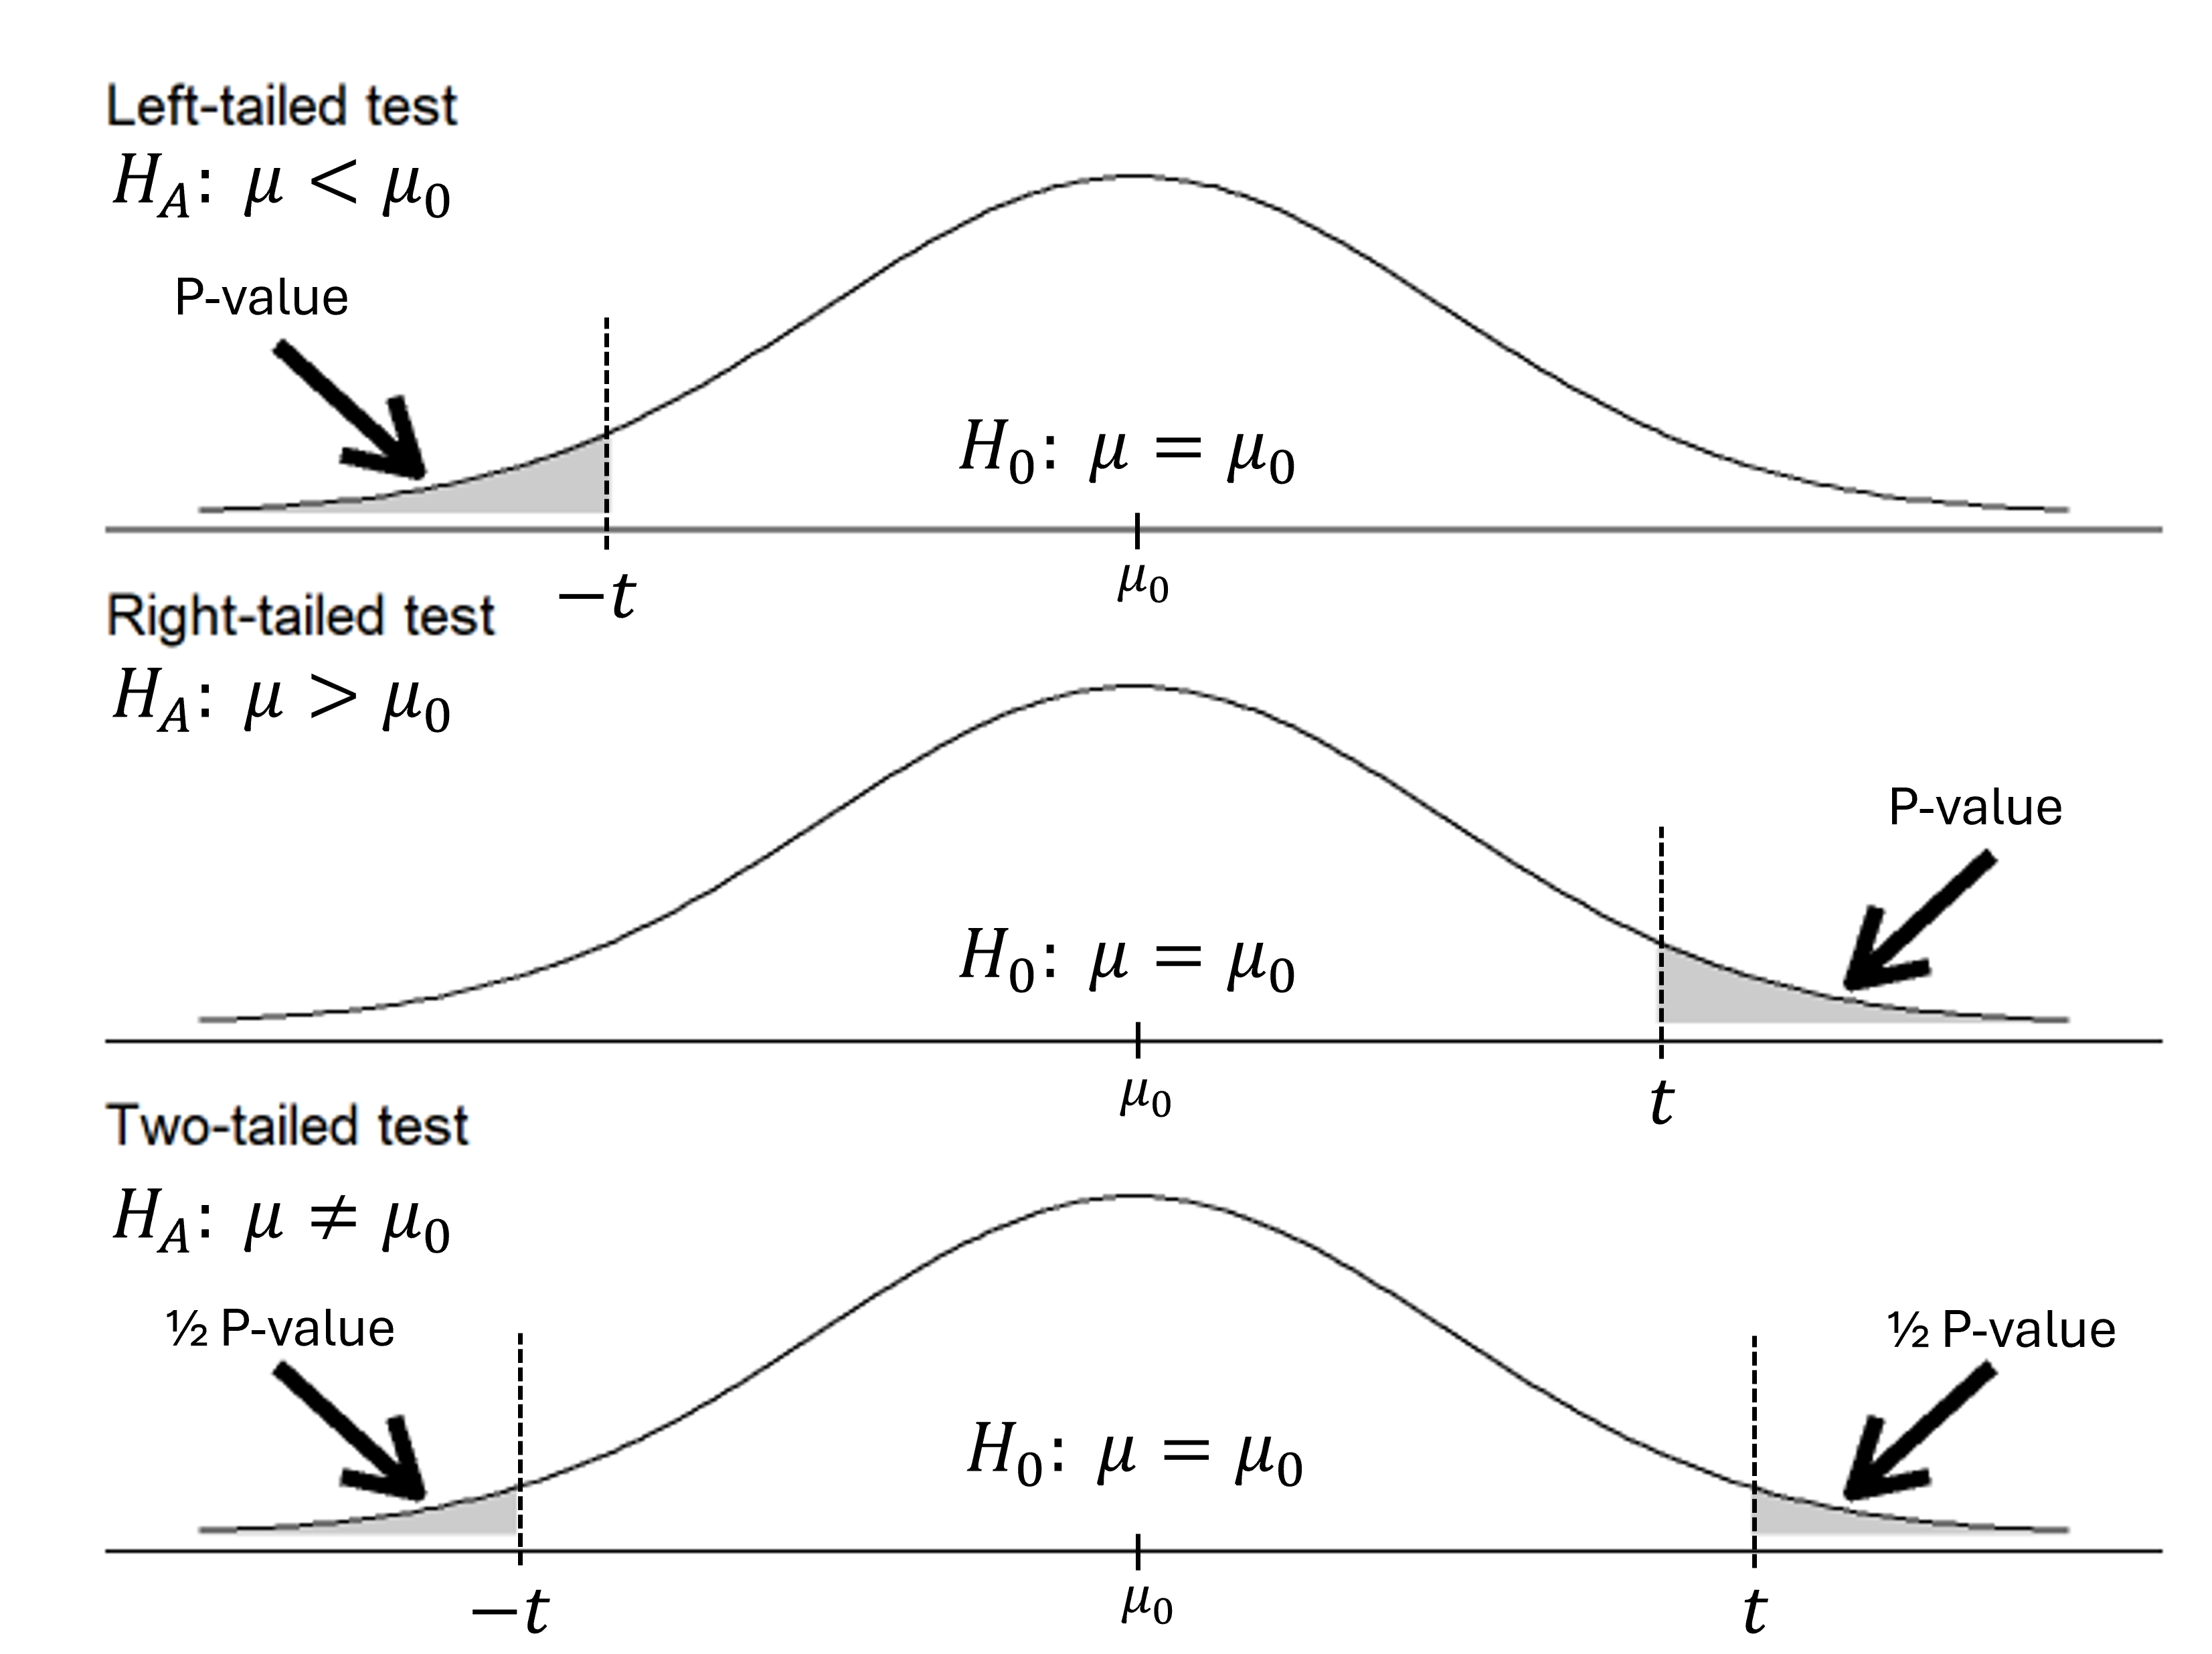
\includegraphics{cheatsheet_files/mediabag/one-sample-t-test.png}

The test statistic \(t\) (the \(t\)-statistic) calculates how many
standard errors (\(\text{SE}_{\bar{x}}\)) away from the null hypothesis
\(\mu_0\) that the observed statistic \(\bar{x}\) is.

\[
t=\frac{\bar{x}-\mu_0}{\text{SE}_{\bar{x}}}=\frac{\bar{x}-\mu_0}{\frac{s}{\sqrt{n}}}
\]

The \(t\)-statistic is used to find the probability of your sample
having the mean \(\bar{x}\) if the null distribution
\(\text{N}\left(\mu_0, \text{SE}_{\bar{x}_0}\right)\) were the ``true''
distribution in your population.

The probability of the sample statistic \(\bar{x}\) under the null
hypothesis \(\mu=\mu_0\) and
\(\bar{x} \sim \text{N}\left(\mu_0, \text{SE}_{\bar{x}}\right)\) is
calculated from the \(t\) distribution in R using the function
\texttt{pt()}. This function takes the test statistic \(t\) (called
\texttt{q} or quantile in R) and the degrees of freedom \texttt{df}
(\(n-1\)) as parameters. This probability is known as the p-value.

\begin{Shaded}
\begin{Highlighting}[]
\CommentTok{\# left{-}tailed hypothesis test}
\FunctionTok{pt}\NormalTok{(}\SpecialCharTok{{-}}\NormalTok{t, }\AttributeTok{df=}\NormalTok{n}\DecValTok{{-}1}\NormalTok{)}

\CommentTok{\# right{-}tailed hypothesis test}
\FunctionTok{pt}\NormalTok{(t, }\AttributeTok{df=}\NormalTok{n}\DecValTok{{-}1}\NormalTok{, }\AttributeTok{lower.tail=}\NormalTok{F)}

\CommentTok{\# two{-}tailed hypothesis test}
\FunctionTok{pt}\NormalTok{(}\SpecialCharTok{{-}}\NormalTok{t, }\AttributeTok{df=}\NormalTok{n}\DecValTok{{-}1}\NormalTok{)}\SpecialCharTok{*}\DecValTok{2}
\FunctionTok{pt}\NormalTok{(t, }\AttributeTok{df=}\NormalTok{n}\DecValTok{{-}1}\NormalTok{, }\AttributeTok{lower.tail=}\NormalTok{F)}\SpecialCharTok{*}\DecValTok{2}
\FunctionTok{pt}\NormalTok{(}\SpecialCharTok{{-}}\NormalTok{t, }\AttributeTok{df=}\NormalTok{n}\DecValTok{{-}1}\NormalTok{)}\SpecialCharTok{+}\FunctionTok{pt}\NormalTok{(t, }\AttributeTok{df=}\NormalTok{n}\DecValTok{{-}1}\NormalTok{, }\AttributeTok{lower.tail=}\NormalTok{F)}
\end{Highlighting}
\end{Shaded}

A small p-value indicates that the probability of taking a sample of
size \(n\) with your observed sample mean \(\bar{x}\) from the null
sampling distribution
\(\bar{x}_0 \sim \text{N}\left(\mu_0, \text{SE}_{\bar{x}_0}\right)\) is
very low.

If the p-value for your \(t\)-statistic is less than your significance
threshold \(\alpha\) (i.e.~the Type I Error Rate), then this is
sufficient evidence that the null hypothesis \(H_0 \colon \mu=\mu_0\)
may not be true. Reject the null hypothesis \(H_0\) and accept the
alternate hypothesis \(H_A\).

If the p-value for your \(t\)-statistic is greater than \(\alpha\), this
is not sufficient evidence against the null hypothesis
\(H_0 \colon \mu=\mu_0\). You fail to reject the null hypothesis
\(H_0\).

\subsubsection{Paired Means}\label{paired-means}

\begin{itemize}
\item
  A \textbf{\emph{paired means}} \(t\)-test is a special instance of a
  1-sample \(t\)-test. It tests if the mean of the difference between 2
  paired measures (\(\mu_{\text{difference}}\)) in a population is
  different from a null value (\(\mu_0\)). Typically, \(\mu_0=0\).
\item
  Sample statistics mean \(\bar{x}_{\text{difference}}\) and standard
  deviation \(s_{\text{difference}}\) are calculated using the
  difference between the 2 paired measures
  \(x_{\text{difference}}=x_1-x_2\), not the individual measures \(x_1\)
  or \(x_2\).
\item
  Sample statistics \(\bar{x}_{\text{difference}}\) (mean) and
  \(s_{\text{difference}}\) (standard deviation) and the sample size
  \(n\) are used to infer the sampling distribution of the mean
  \(\bar{x}_{\text{difference}} \sim \operatorname{N}\left(\mu_{\text{difference}}, SE_{\bar{x}_{\text{difference}}}\right)\).
\item
  To account for using \(s \approx \sigma\) in the standard error,
  confidence intervals and hypothesis tests are based on the \(T\)
  distribution (Student's \(t\)) with the parameter
  \(\text{degrees of freedom (df)}=n-1\).
\end{itemize}

\paragraph{Confidence Interval}\label{confidence-interval-1}

The confidence interval for the population difference in paired means
\(\mu_{\text{difference}}\) is calculated using the point estimate
\(\bar{x}_{\text{difference}}\).

\[
\bar{x}_{\text{difference}} \pm T_{\text{df}}^* \times SE_{\bar{x}_{\text{difference}}}
\]

The standard error of \(\bar{x}_{\text{difference}}\) is estimated from
the observed standard deviation \(s_{\text{difference}}\) and the sample
size \(n\).

\[
\operatorname{SE}_{\bar{x}_{\text{difference}}}=\frac{\sigma_{\text{difference}}}{\sqrt{n}}\approx\frac{s_{\text{difference}}}{\sqrt{n}}
\]

The critical value from the \(t\) distribution with degrees of freedom
\(\text{df}=n-1\) is\ldots{}

\[
T_{\text{df}}^*=T_{\text{df},\alpha/2}=T_{\text{df}, 1-\alpha/2}
\]

A critical value is calculated from the \(t\) distribution in R using
the function \texttt{qt()}. This function takes a probability \texttt{p}
(\(\alpha/2\) or \(1-\alpha/2\)) and degrees of freedom \texttt{df}
(\(n-1\)).

\begin{Shaded}
\begin{Highlighting}[]
\FunctionTok{qt}\NormalTok{(alpha}\SpecialCharTok{/}\DecValTok{2}\NormalTok{, }\AttributeTok{df=}\NormalTok{n}\DecValTok{{-}1}\NormalTok{)}

\FunctionTok{qt}\NormalTok{(}\DecValTok{1}\SpecialCharTok{{-}}\NormalTok{alpha}\SpecialCharTok{/}\DecValTok{2}\NormalTok{, }\AttributeTok{df=}\NormalTok{n}\DecValTok{{-}1}\NormalTok{)}
\end{Highlighting}
\end{Shaded}

\paragraph{Hypothesis Test}\label{hypothesis-test-1}

The null hypothesis for a paired means \(t\)-test states that the
population mean \(\mu_{\text{difference}}\) is equal to some null value
\(\mu_0\). Typically, \(\mu_0=0\).

\[
H_0 \colon \mu_{\text{difference}}=\mu_0
\]

The null distribution of the sample mean
\(\bar{x}_{\text{difference0}}\), given the null hypothesis that
\(\mu_{\text{difference}}=\mu_0\), is
\(\bar{x}_{\text{difference0}} \sim \text{N}\left(\mu_0, SE_{\bar{x}_{\text{difference}}}\right)\).
The standard error of the null sample mean
\(\bar{x}_{\text{difference0}}\) is the same as the standard error of
the observed sample mean \(\bar{x}_{\text{difference}}\).

\[
\text{SE}_{\bar{x}_{\text{difference0}}}=\text{SE}_{\bar{x}_{\text{difference}}}=\frac{\sigma_{\text{difference}}}{\sqrt{n}} \approx \frac{s_{\text{difference}}}{\sqrt{n}}
\]

A confidence interval for the null population mean
\(\mu_{\text{difference}}\) under the null hypothesis
\(H_0 \colon \mu_{\text{difference}}=\mu_0\) is calculated using
\(\mu_0\) as the point estimate.

\[
\mu_0 \pm T_{\text{df}}^* \times \text{SE}_{\bar{x}_{\text{difference}}}
\]

The alternate hypothesis of a 1-sample \(t\)-test states that the
population mean \(\mu_{\text{difference}}\) is greater than, less than,
or not equal to some null value \(\mu_0\).

\begin{itemize}
\item
  \(H_A \colon \mu_{\text{difference}} < \mu_0\), left-tailed test
  (one-sided)
\item
  \(H_A \colon \mu_{\text{difference}} > \mu_0\), right-tailed test
  (one-sided)
\item
  \(H_A \colon \mu_{\text{difference}} \ne \mu_0\), two-tailed test
  (two-sided)
\end{itemize}

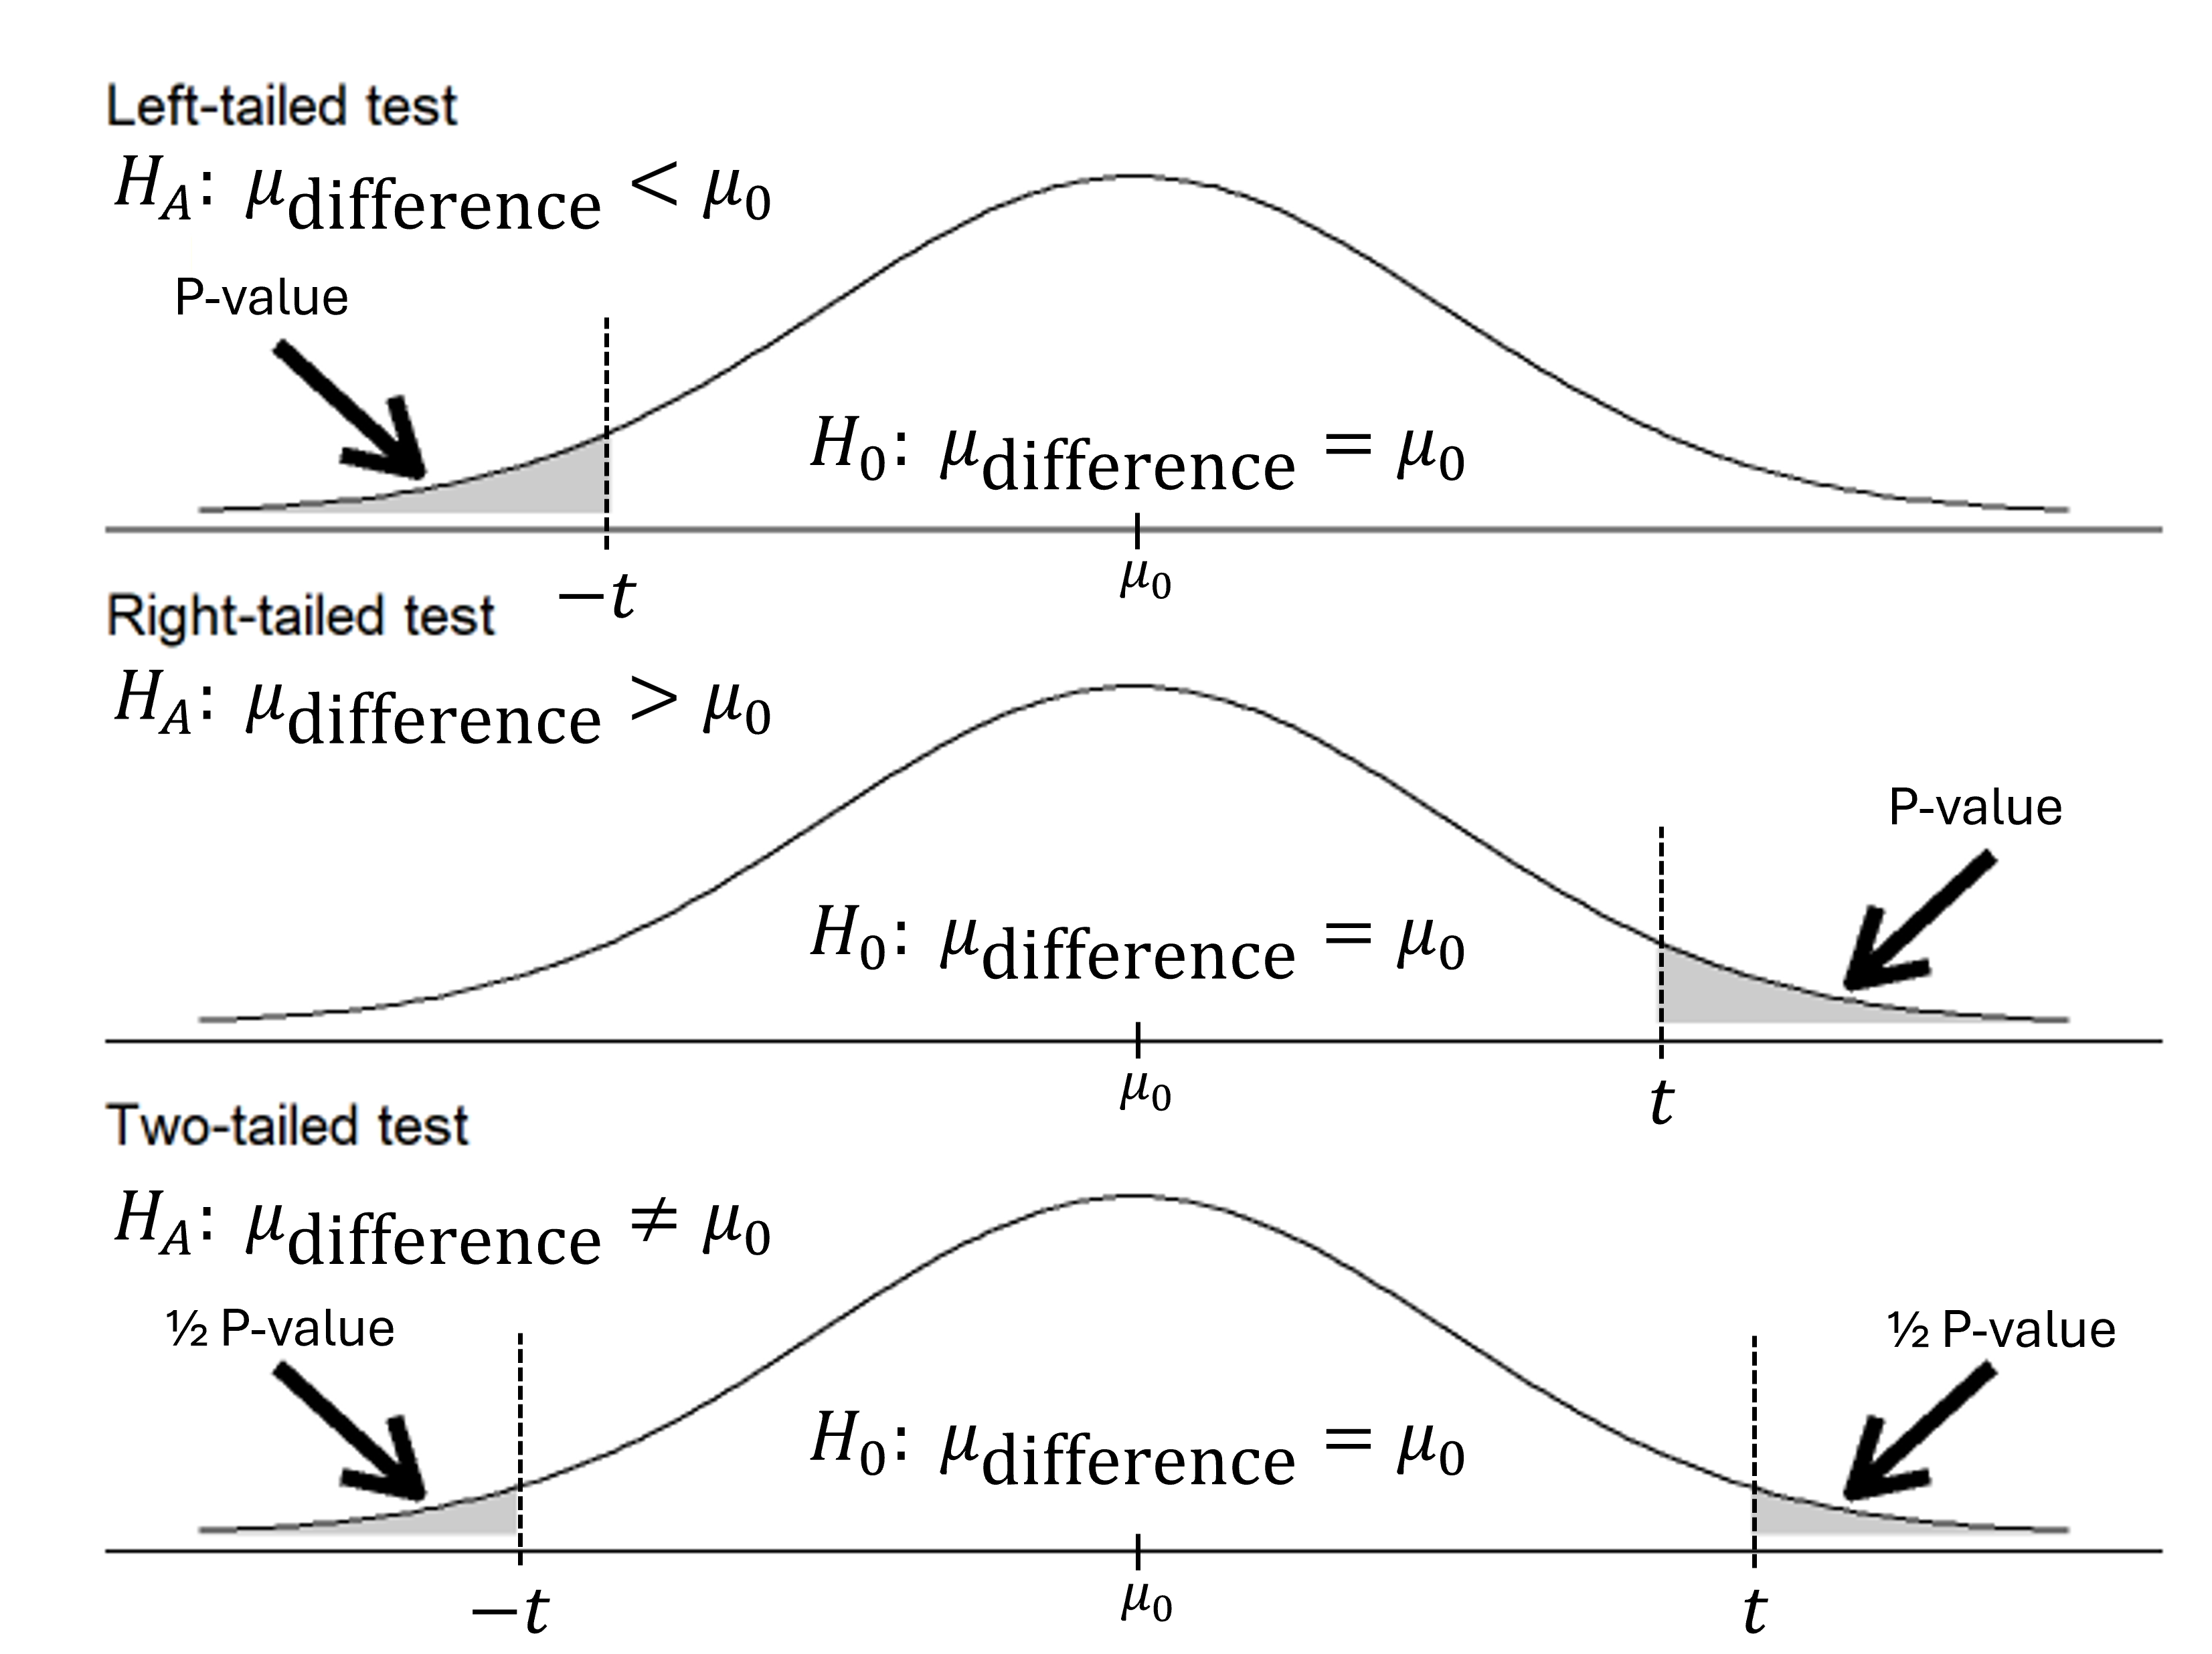
\includegraphics{cheatsheet_files/mediabag/paired-means-t-test.png}

The test statistic \(t\) (the \(t\)-statistic) calculates how many
standard errors (\(\text{SE}_{\bar{x}_{\text{difference}}}\)) away from
the null hypothesis \(\mu_0\) that the observed statistic
\(\bar{x}_{\text{difference}}\) is.

\[
t=\frac{\bar{x}_{\text{difference}}-\mu_0}{\text{SE}_{\bar{x}_{\text{difference}}}}=\frac{\bar{x}_{\text{difference}}-\mu_0}{\frac{s_{\text{difference}}}{\sqrt{n}}}
\]

The \(t\)-statistic is used to find the probability of your sample
having the mean \(\bar{x}_{\text{difference}}\) if the null distribution
\(\text{N}\left(\mu_0, \text{SE}_{\bar{x}_{\text{difference}}}\right)\)
were the ``true'' distribution in your population for
\(\bar{x}_{\text{difference}}\).

The probability of the sample statistic \(\bar{x}_{\text{difference}}\)
under the null hypothesis \(\mu_{\text{difference}}=\mu_0\) and
\(\bar{x}_{\text{difference0}} \sim \text{N}\left(\mu_0, \text{SE}_{\bar{x}_{\text{difference}}}\right)\)
is calculated from the \(t\) distribution in R using the function
\texttt{pt()}. This function takes the test statistic \(t\) (called
\texttt{q} or quantile in R) and the degrees of freedom \texttt{df}
(\(n-1\)) as parameters. This probability is known as the p-value.

\begin{Shaded}
\begin{Highlighting}[]
\CommentTok{\# left{-}tailed hypothesis test}
\FunctionTok{pt}\NormalTok{(}\SpecialCharTok{{-}}\NormalTok{t, }\AttributeTok{df=}\NormalTok{n}\DecValTok{{-}1}\NormalTok{)}

\CommentTok{\# right{-}tailed hypothesis test}
\FunctionTok{pt}\NormalTok{(t, }\AttributeTok{df=}\NormalTok{n}\DecValTok{{-}1}\NormalTok{, }\AttributeTok{lower.tail=}\NormalTok{F)}

\CommentTok{\# two{-}tailed hypothesis test}
\FunctionTok{pt}\NormalTok{(}\SpecialCharTok{{-}}\NormalTok{t, }\AttributeTok{df=}\NormalTok{n}\DecValTok{{-}1}\NormalTok{)}\SpecialCharTok{*}\DecValTok{2}
\FunctionTok{pt}\NormalTok{(t, }\AttributeTok{df=}\NormalTok{n}\DecValTok{{-}1}\NormalTok{, }\AttributeTok{lower.tail=}\NormalTok{F)}\SpecialCharTok{*}\DecValTok{2}
\FunctionTok{pt}\NormalTok{(}\SpecialCharTok{{-}}\NormalTok{t, }\AttributeTok{df=}\NormalTok{n}\DecValTok{{-}1}\NormalTok{)}\SpecialCharTok{+}\FunctionTok{pt}\NormalTok{(t, }\AttributeTok{df=}\NormalTok{n}\DecValTok{{-}1}\NormalTok{, }\AttributeTok{lower.tail=}\NormalTok{F)}
\end{Highlighting}
\end{Shaded}

A small p-value indicates that the probability of taking a sample of
size \(n\) with your observed sample mean
\(\bar{x}_{\text{difference}}\) from the null sampling distribution
\(\bar{x}_{\text{difference0}} \sim \text{N}\left(\mu_0, \text{SE}_{\bar{x}_{\text{difference}}}\right)\)
is very low.

If the p-value for your \(t\)-statistic is less than your significance
threshold \(\alpha\) (i.e.~the Type I Error Rate), then this is
sufficient evidence that the null hypothesis
\(H_0 \colon \mu_{\text{difference}}=\mu_0\) may not be true. Reject the
null hypothesis \(H_0\) and accept the alternate hypothesis \(H_A\).

If the p-value for your \(t\)-statistic is greater than \(\alpha\), this
is not sufficient evidence against the null hypothesis
\(H_0 \colon \mu_{\text{difference}}=\mu_0\). You fail to reject the
null hypothesis \(H_0\).

\subsubsection{Two Means}\label{two-means}

\begin{itemize}
\item
  A \textbf{\emph{2-sample}} \(t\)-test tests if the difference between
  2 means (\(\mu_1-\mu_2\)) of a population is different from a null
  value (\(\mu_0\)). Often, \(\mu_0=0\).
\item
  Sample statistics \(\bar{x}_1-\bar{x}_2\) (difference in means),
  standard deviations (\(s_1\) and \(s_2\)), and the sample sizes
  \(n_1\) and \(n_2\) are used to infer the sampling distribution of the
  difference in means
  \(\bar{x}_1-\bar{x}_2 \sim \operatorname{N}\left(\mu_1-\mu_2, SE_{\bar{x}_1-\bar{x}_2}\right)\).
\item
  To account for using \(s \approx \sigma\) in the standard error,
  confidence intervals and hypothesis tests are based on the \(T\)
  distribution (Student's \(t\)) with the parameter
  \(\text{degrees of freedom (df)}=\text{min}(n_1, n_2)-1\).
\end{itemize}

\paragraph{Confidence Interval}\label{confidence-interval-2}

The confidence interval for a difference in means \(\mu_1-\mu_2\) is
calculated using the point estimate \(\bar{x}_1-\bar{x}_2\).

\[
\bar{x}_1-\bar{x}_2 \pm T_{\text{df}}^* \times SE_{\bar{x}_1-\bar{x}_2}
\]

The standard error of \(\bar{x}_1-\bar{x}_2\) is estimated from the 2
observed standard deviations \(s_1\) and \(s_2\) and the 2 sample sizes
\(n_1\) and \(n_2\).

\[
\operatorname{SE}_{\bar{x}_1-\bar{x}_2}=  \sqrt{\frac{\sigma_1^2}{n_1}+\frac{\sigma_2^2}{n_2}} \approx \sqrt{\frac{s_1^2}{n_1}+\frac{s_2^2}{n_2}}
\]

The critical value from the \(t\) distribution with degrees of freedom
\(\text{df}=\text{minimum}(n_1, n_2)-1\) is\ldots{}

\[
T_{\text{df}}^*=T_{\text{df},\alpha/2}=T_{\text{df}, 1-\alpha/2}
\]

A critical value is calculated from the \(t\) distribution in R using
the function \texttt{qt()}. This function takes a probability \texttt{p}
(\(\alpha/2\) or \(1-\alpha/2\)) and degrees of freedom \texttt{df}
(\(\text{minimum}(n_1, n_2)-1\)).

\begin{Shaded}
\begin{Highlighting}[]
\FunctionTok{qt}\NormalTok{(alpha}\SpecialCharTok{/}\DecValTok{2}\NormalTok{, }\AttributeTok{df=}\FunctionTok{min}\NormalTok{(n1, n2)}\SpecialCharTok{{-}}\DecValTok{1}\NormalTok{)}

\FunctionTok{qt}\NormalTok{(}\DecValTok{1}\SpecialCharTok{{-}}\NormalTok{alpha}\SpecialCharTok{/}\DecValTok{2}\NormalTok{, }\AttributeTok{df=}\FunctionTok{min}\NormalTok{(n1, n2)}\SpecialCharTok{{-}}\DecValTok{1}\NormalTok{)}
\end{Highlighting}
\end{Shaded}

\paragraph{Hypothesis Test}\label{hypothesis-test-2}

The null hypothesis for a 2-sample \(t\)-test states that the population
difference in means \(\mu_1-\mu_2\) is equal to some null value
\(\mu_0\). Often, \(\mu_0=0\).

\[
H_0 \colon \mu=\mu_0
\]

The null distribution of the difference in sample means
\(\bar{x}_1-\bar{x}_2\), given the null hypothesis that
\(\mu_1-\mu_2=\mu_0\), is
\(\bar{x}_1-\bar{x}_2 \sim \text{N}\left(\mu_0, SE_{\bar{x}_1-\bar{x}_2}\right)\).
The standard error of the null difference in sample means
\(\bar{x}_1-\bar{x}_2\) is the same as the standard error of the
observed difference in sample means.

\[
\text{SE}_{\bar{x}_1-\bar{x}_2}=\sqrt{\frac{\sigma_1^2}{n_1}+\frac{\sigma_2^2}{n_2}} \approx \sqrt{\frac{s_1^2}{n_1}+\frac{s_2^2}{n_2}}
\]

A confidence interval for the null difference in population means
\(\mu_1-\mu_2\) under the null hypothesis
\(H_0 \colon \mu_1-\mu_2=\mu_0\) is calculated using \(\mu_0\) as the
point estimate.

\[
\mu_0 \pm T_{\text{df}}^* \times \text{SE}_{\bar{x}_1-\bar{x}_2}
\]

The alternate hypothesis of a 2-sample \(t\)-test states that the
population difference in means \(\mu_1-\mu_2\) is greater than, less
than, or not equal to some null value \(\mu_0\).

\begin{itemize}
\item
  \(H_A \colon \mu_1-\mu_2 < \mu_0\), left-tailed test (one-sided)
\item
  \(H_A \colon \mu_1-\mu_2 > \mu_0\), right-tailed test (one-sided)
\item
  \(H_A \colon \mu_1-\mu_2 \ne \mu_0\), two-tailed test (two-sided)
\end{itemize}

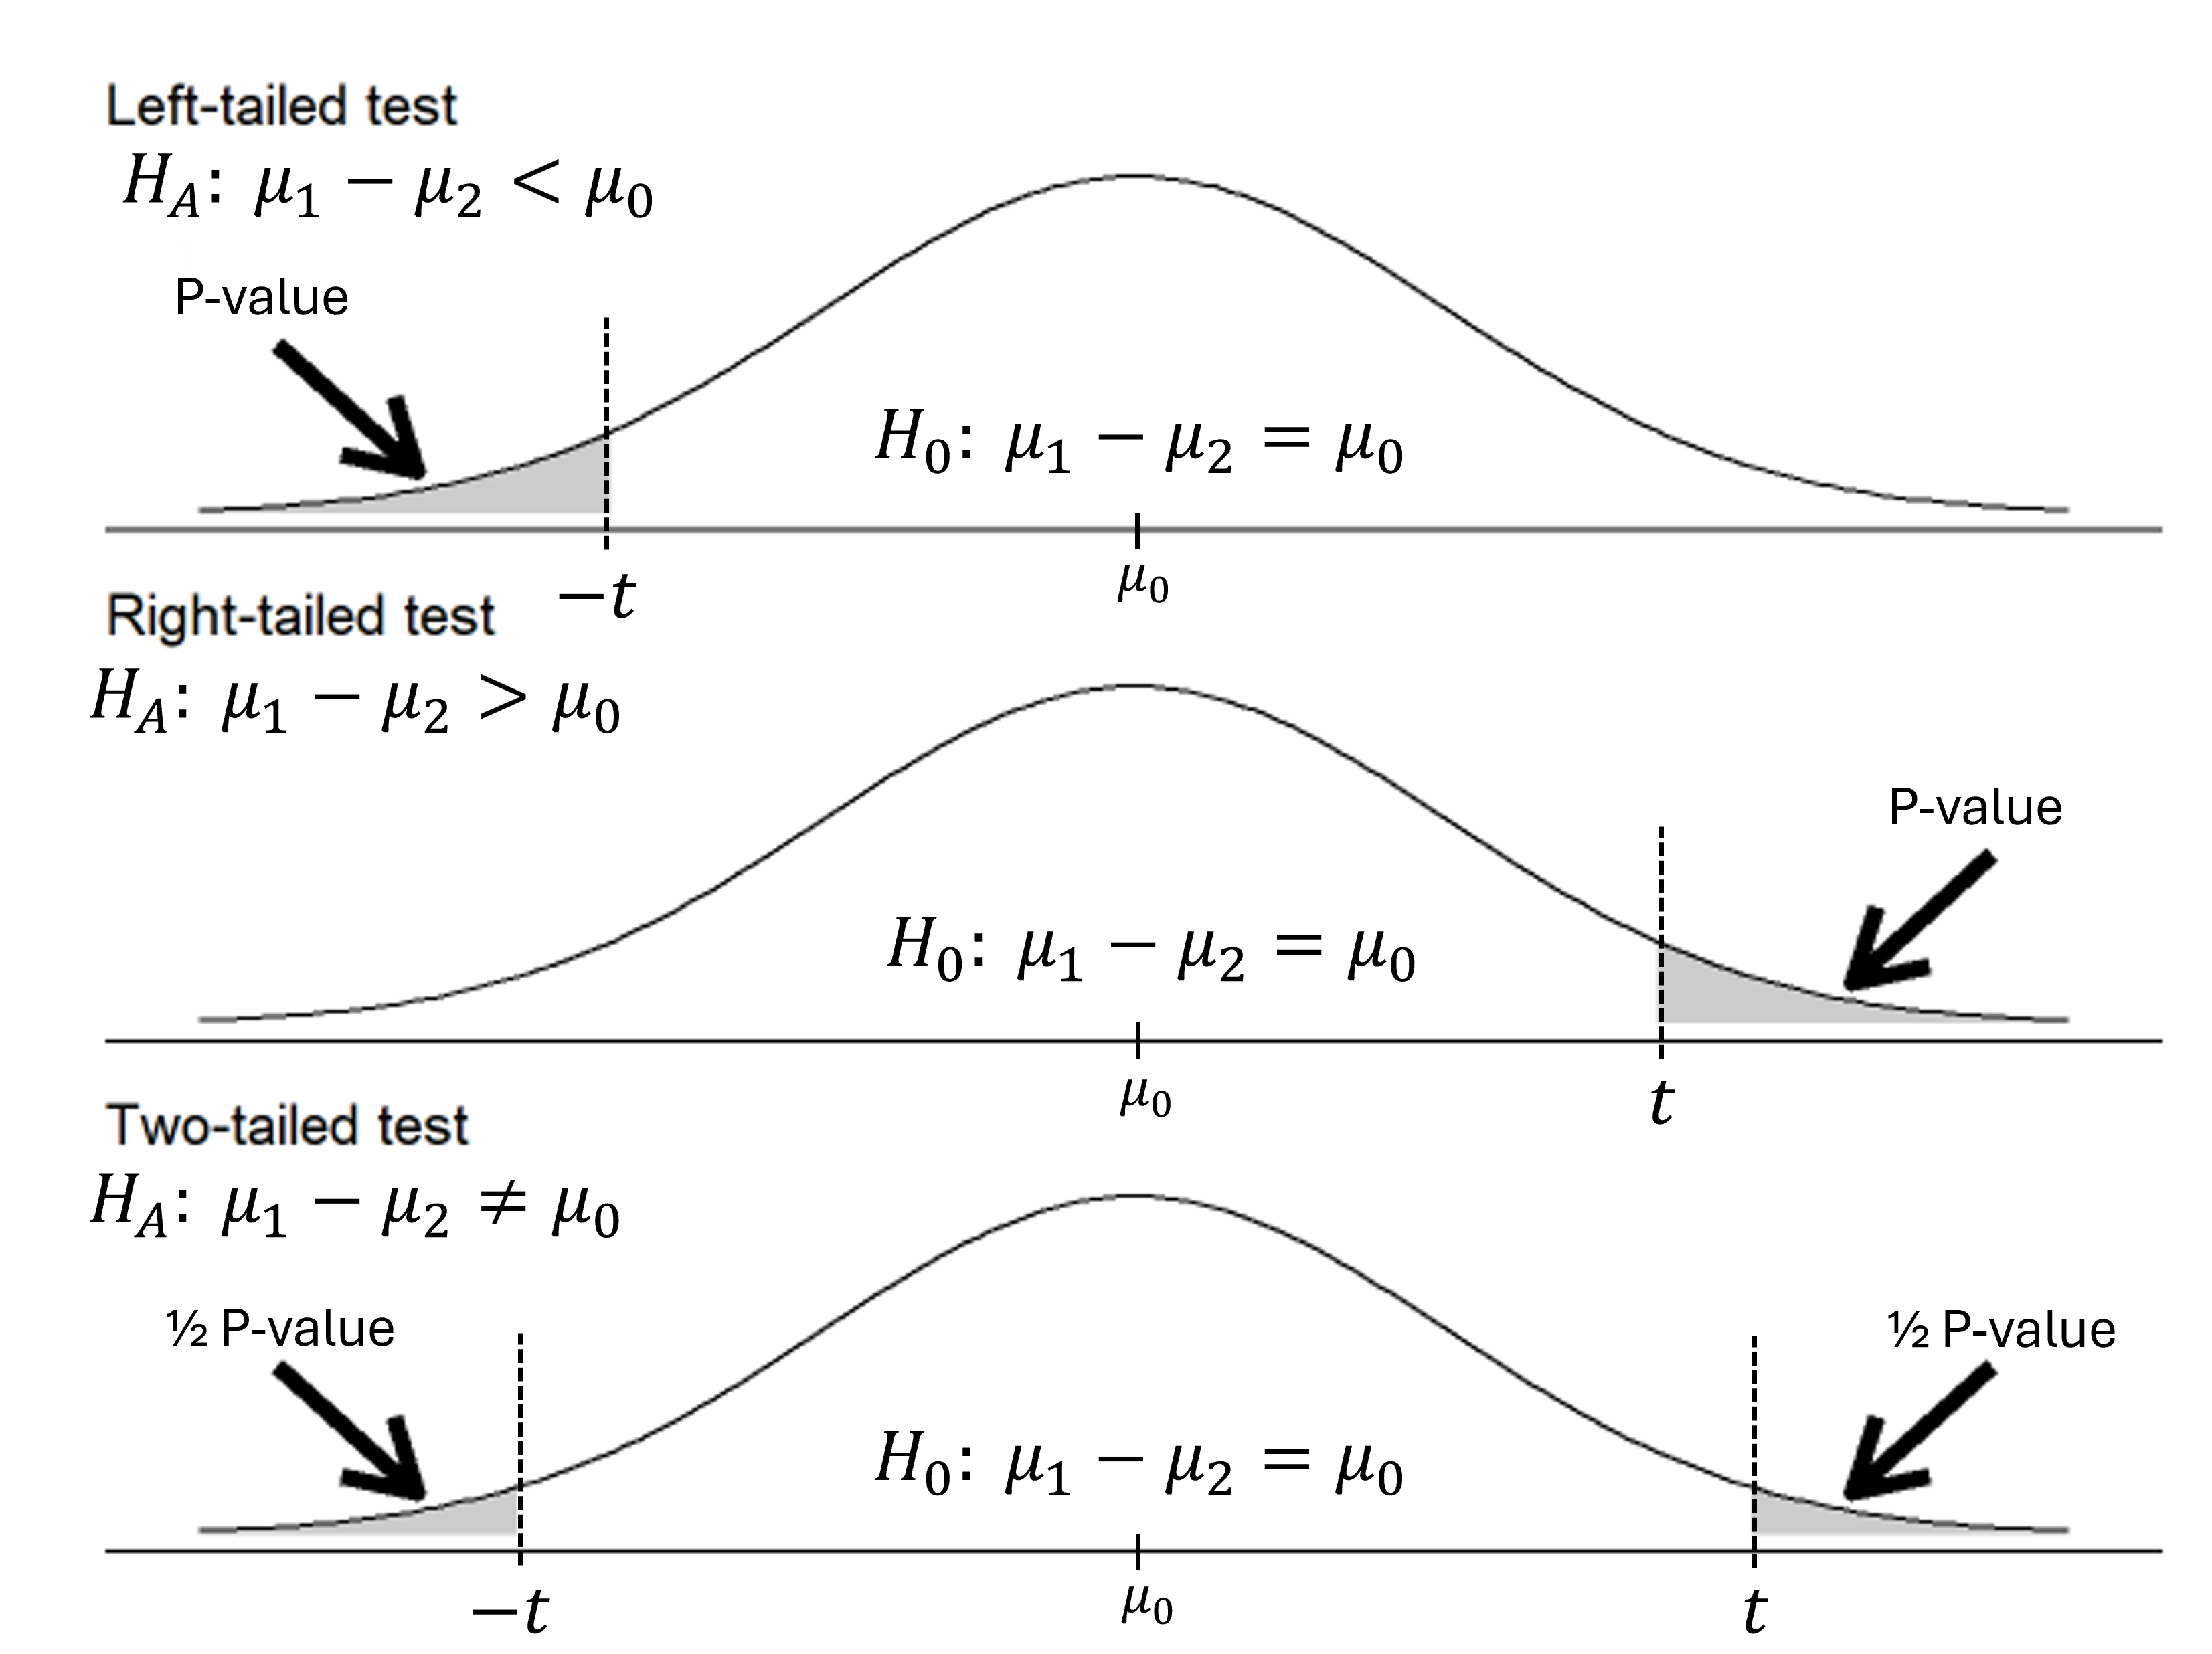
\includegraphics{cheatsheet_files/mediabag/two-sample-t-test.png}

The test statistic \(t\) (the \(t\)-statistic) calculates how many
standard errors (\(\text{SE}_{\bar{x}_1-\bar{x}_2}\)) away from the null
hypothesis \(\mu_0\) that the observed statistic \(\bar{x}_1-\bar{x}_2\)
is.

\[
t=\frac{(\bar{x}_1-\bar{x}_2)-\mu_0}{\text{SE}_{\bar{x}_1-\bar{x}_2}}=\frac{(\bar{x}_1-\bar{x}_2)-\mu_0}{\sqrt{\frac{s_1^2}{n_1}+\frac{s_2^2}{n_2}}}
\]

When the null hypothesis is that the population difference in means is 0
(\(H_0 \colon \mu_1-\mu_2=0\)), the calculation for the test statistic
simplifies to the below.

\[
t=\frac{\bar{x}_1-\bar{x}_2}{\text{SE}_{\bar{x}_1-\bar{x}_2}}=\frac{\bar{x}_1-\bar{x}_2}{\sqrt{\frac{s_1^2}{n_1}+\frac{s_2^2}{n_2}}}
\]

The \(t\)-statistic is used to find the probability of your sample
having the difference in means \(\bar{x}_1-\bar{x}_2\) if the null
distribution
\(\text{N}\left(\mu_0, \text{SE}_{\bar{x}_1-\bar{x}_2}\right)\) were the
``true'' distribution in your population.

The probability of the sample statistic \(\bar{x}_1-\bar{x}_2\) under
the null hypothesis \(\mu_1-\mu_2=\mu_0\) and
\(\bar{x}_1-\bar{x}_2 \sim \text{N}\left(\mu_0, \text{SE}_{\bar{x}_1-\bar{x}_2}\right)\)
is calculated from the \(t\) distribution in R using the function
\texttt{pt()}. This function takes the test statistic \(t\) (called
\texttt{q} or quantile in R) and the degrees of freedom \texttt{df}
(\(\text{minimum}(n_1, n_2)-1\)) as parameters. This probability is
known as the p-value.

\begin{Shaded}
\begin{Highlighting}[]
\CommentTok{\# left{-}tailed hypothesis test}
\FunctionTok{pt}\NormalTok{(}\SpecialCharTok{{-}}\NormalTok{t, }\AttributeTok{df=}\FunctionTok{min}\NormalTok{(n1, n2)}\SpecialCharTok{{-}}\DecValTok{1}\NormalTok{)}

\CommentTok{\# right{-}tailed hypothesis test}
\FunctionTok{pt}\NormalTok{(t, }\AttributeTok{df=}\FunctionTok{min}\NormalTok{(n1, n2)}\SpecialCharTok{{-}}\DecValTok{1}\NormalTok{, }\AttributeTok{lower.tail=}\NormalTok{F)}

\CommentTok{\# two{-}tailed hypothesis test}
\FunctionTok{pt}\NormalTok{(}\SpecialCharTok{{-}}\NormalTok{t, }\AttributeTok{df=}\FunctionTok{min}\NormalTok{(n1, n2)}\SpecialCharTok{{-}}\DecValTok{1}\NormalTok{)}\SpecialCharTok{*}\DecValTok{2}
\FunctionTok{pt}\NormalTok{(t, }\AttributeTok{df=}\FunctionTok{min}\NormalTok{(n1, n2)}\SpecialCharTok{{-}}\DecValTok{1}\NormalTok{, }\AttributeTok{lower.tail=}\NormalTok{F)}\SpecialCharTok{*}\DecValTok{2}
\FunctionTok{pt}\NormalTok{(}\SpecialCharTok{{-}}\NormalTok{t, }\AttributeTok{df=}\FunctionTok{min}\NormalTok{(n1, n2)}\SpecialCharTok{{-}}\DecValTok{1}\NormalTok{)}\SpecialCharTok{+}\FunctionTok{pt}\NormalTok{(t, }\AttributeTok{df=}\FunctionTok{min}\NormalTok{(n1, n2)}\SpecialCharTok{{-}}\DecValTok{1}\NormalTok{, }\AttributeTok{lower.tail=}\NormalTok{F)}
\end{Highlighting}
\end{Shaded}

A small p-value indicates that the probability of taking samples of size
\(n_1\) and \(n_2\) with your observed difference in sample means
\(\bar{x}_1-\bar{x}_2\) from the null sampling distribution
\(\bar{x}_1-\bar{x}_2 \sim \text{N}\left(\mu_0, \text{SE}_{\bar{x}_1-\bar{x}_2}\right)\)
is very low.

If the p-value for your \(t\)-statistic is less than your significance
threshold \(\alpha\) (i.e.~the Type I Error Rate), then this is
sufficient evidence that the null hypothesis
\(H_0 \colon \mu_1-\mu_2=\mu_0\) may not be true. Reject the null
hypothesis \(H_0\) and accept the alternate hypothesis \(H_A\).

If the p-value for your \(t\)-statistic is greater than \(\alpha\), this
is not sufficient evidence against the null hypothesis
\(H_0 \colon \mu_1-\mu_2=\mu_0\). You fail to reject the null hypothesis
\(H_0\).

\subsection{Proportions}\label{proportions}

\begin{longtable}[]{@{}
  >{\raggedright\arraybackslash}p{(\columnwidth - 4\tabcolsep) * \real{0.3750}}
  >{\raggedright\arraybackslash}p{(\columnwidth - 4\tabcolsep) * \real{0.3194}}
  >{\raggedright\arraybackslash}p{(\columnwidth - 4\tabcolsep) * \real{0.3056}}@{}}
\caption{Sample Statistics for Inference of Population
Proportions}\tabularnewline
\toprule\noalign{}
\begin{minipage}[b]{\linewidth}\raggedright
Measure
\end{minipage} & \begin{minipage}[b]{\linewidth}\raggedright
Sample Statistic
\end{minipage} & \begin{minipage}[b]{\linewidth}\raggedright
Population Parameter
\end{minipage} \\
\midrule\noalign{}
\endfirsthead
\toprule\noalign{}
\begin{minipage}[b]{\linewidth}\raggedright
Measure
\end{minipage} & \begin{minipage}[b]{\linewidth}\raggedright
Sample Statistic
\end{minipage} & \begin{minipage}[b]{\linewidth}\raggedright
Population Parameter
\end{minipage} \\
\midrule\noalign{}
\endhead
\bottomrule\noalign{}
\endlastfoot
Proportion & \(\hat{p}\) & \(p\) \\
Difference in Proportions & \(\hat{p}_1-\hat{p}_2\) & \(p_1-p_2\) \\
\end{longtable}

\subsubsection{Assumptions}\label{assumptions-1}

\begin{itemize}
\item
  \textbf{\emph{Independence}}: sample observations are independent
  (i.e.~random sample).
\item
  \textbf{\emph{Sample size}}: the sample size should be greater than 20
  (\(n \ge 20\)) with at least 10 successes (\(np \ge 10\)) and 10
  failures (\(n(1-p) \ge 10\)).
\item
  \textbf{\emph{Validity}}: sample statistics approximate the population
  parameters (\(\bar{x} \approx \mu\), \(s \approx \sigma\))
\end{itemize}

\subsubsection{\texorpdfstring{Single Proportion (\(\hat{p}\)) -
One-Sample
\(Z\)-test}{Single Proportion (\textbackslash hat\{p\}) - One-Sample Z-test}}\label{single-proportion-hatp---one-sample-z-test}

\begin{itemize}
\item
  A \textbf{\emph{1-sample}} \(Z\)-test tests if the mean proportion
  (\(p\)) for a population is different from a null value (\(p_0\)).
\item
  Sample statistic \(\hat{p}\) (proportion) and sample size \(n\) are
  used to infer the sampling distribution of the mean proportion
  \(\hat{p} \sim \operatorname{N}\left(p, SE_{\hat{p}}\right)\).
\item
  Confidence intervals and hypothesis tests for proportions are based on
  the \(Z\) distribution (standard normal).
\end{itemize}

\paragraph{Confidence Interval}\label{confidence-interval-3}

The confidence interval for a population proportion \(p\) is estimated
from the sample proportion \(\hat{p}\).

\[
\hat{p} \pm Z^* \times SE_{\hat{p}}
\]

The standard error of \(\hat{p}\) is estimated from the sample
proportion \(\hat{p}\) and the sample size \(n\).

\[
\operatorname{SE}_{\hat{p}}=\sqrt{\frac{p(1-p)}{n}}\approx\sqrt{\frac{\hat{p}(1-\hat{p})}{n}}
\]

The critical value from the \(Z\) distribution is\ldots{}

\[
Z^*=Z_{\alpha/2}=Z_{1-\alpha/2}
\]

A critical value is calculated from the \(Z\) distribution in R using
the function \texttt{qnorm()}. This function takes a probability
\texttt{p} (\(\alpha/2\) or \(1-\alpha/2\)), a \texttt{mean} (default =
0), and a standard deviation (\texttt{sd}, default = 1). However, you do
not need to include the \texttt{mean} and \texttt{sd} parameters when
you are using the default standard normal (\(Z\)) distribution.

\begin{Shaded}
\begin{Highlighting}[]
\FunctionTok{qnorm}\NormalTok{(alpha}\SpecialCharTok{/}\DecValTok{2}\NormalTok{)}

\FunctionTok{qnorm}\NormalTok{(}\DecValTok{1}\SpecialCharTok{{-}}\NormalTok{alpha}\SpecialCharTok{/}\DecValTok{2}\NormalTok{)}
\end{Highlighting}
\end{Shaded}

\paragraph{Hypothesis Test}\label{hypothesis-test-3}

The null hypothesis of a 1-sample proportion- or \(Z\)-test states that
the population proportion \(p\) is equal to some null value \(p_0\).

\[
H_0 \colon p=p_0
\]

The null distribution of the sample proportion \(\hat{p}_0\), given the
null hypothesis \(H_0 \colon p=p_0\), is
\(\hat{p} \sim \text{N}\left(p_0, SE_{p_0}\right)\). The standard error
of the null sample proportion \(\hat{p}_0\) under the null hypothesis
\(H_0 \colon p=p_0\) is estimated using the null hypothesis value
\(p_0\) and the sample size \(n\).

\[
\text{SE}_{\hat{p}_0}=\sqrt{\frac{p_0(1-p_0)}{n}}
\]

A confidence interval for the mean proportion under the null hypothesis
is calculated using \(p_0\) as the point estimate and
\(\text{SE}_{\hat{p}_0}\) under the null hypothesis.

\[
p_0 \pm Z^* \times \text{SE}_{\hat{p}_0}
\]

The alternate hypothesis of a 1-sample \(Z\)-test states that the
population proportion \(p\) is greater than, less than, or not equal to
some null value \(p_0\).

\begin{itemize}
\item
  \(H_A \colon p < p_0\), left-tailed test (one-sided)
\item
  \(H_A \colon p > p_0\), right-tailed test (one-sided)
\item
  \(H_A \colon p \ne p_0\), two-tailed test (two-sided)
\end{itemize}

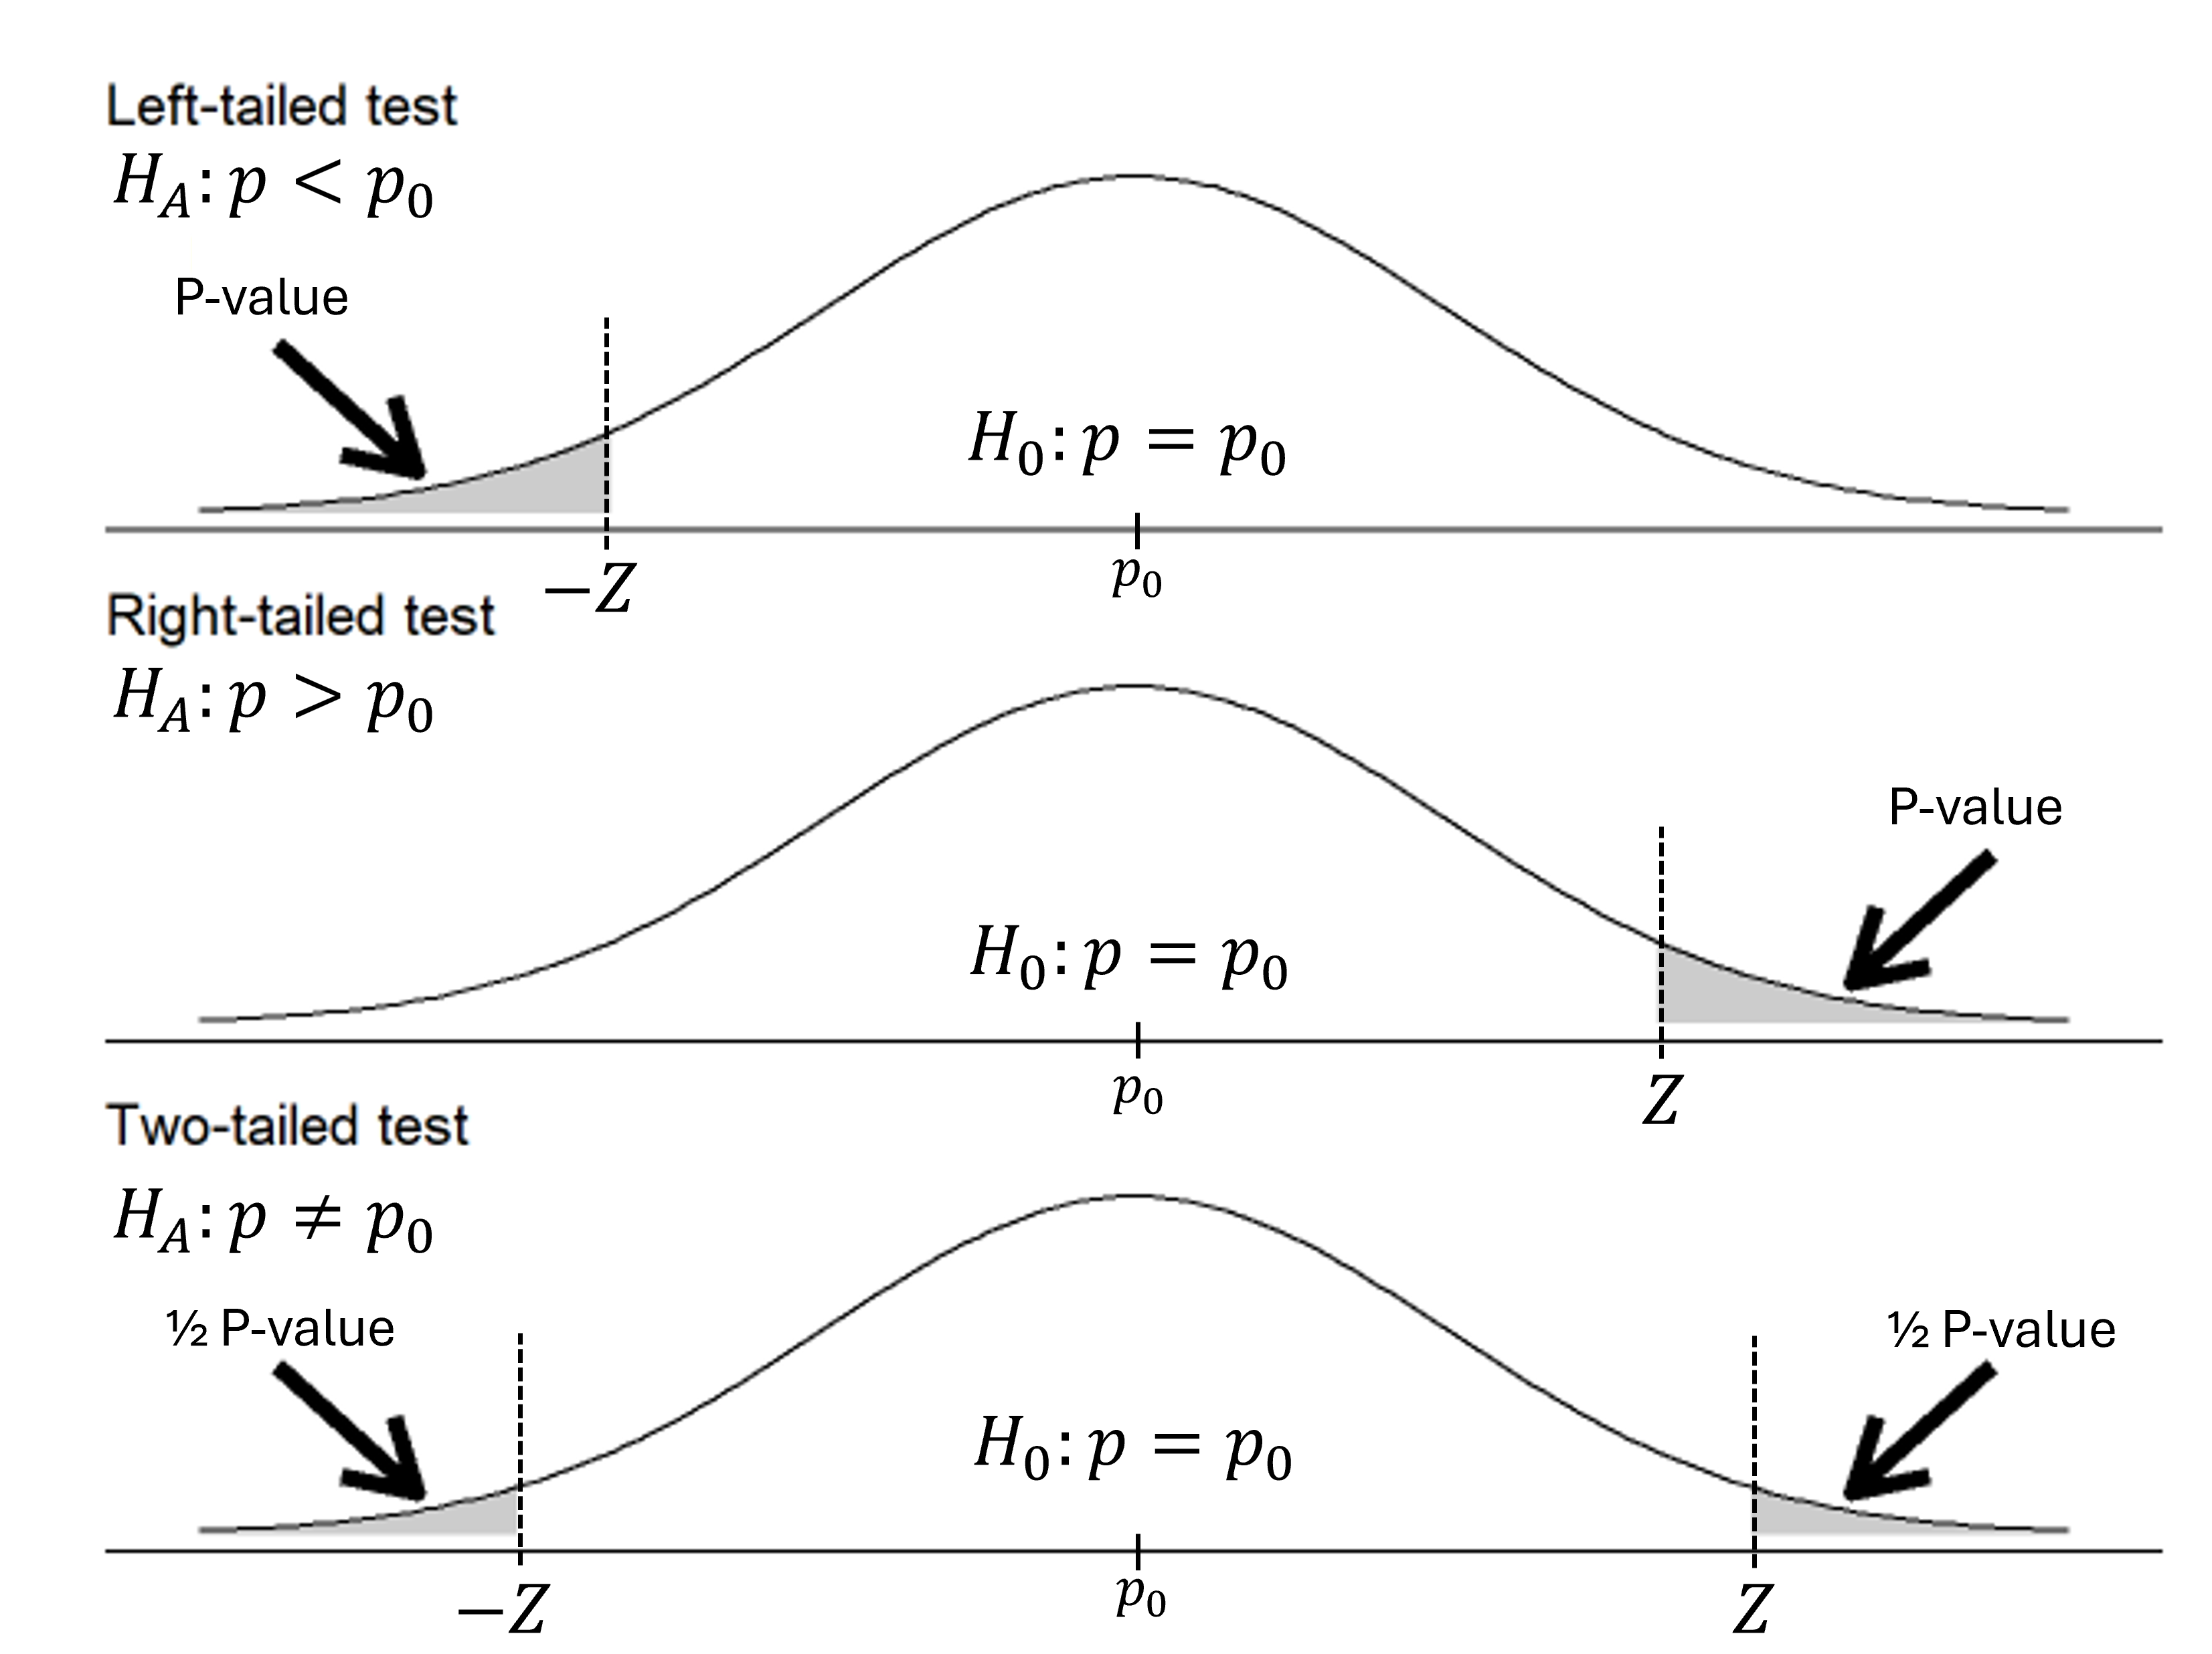
\includegraphics{cheatsheet_files/mediabag/one-sample-prop-test.png}

The test statistic \(Z\) (the \(Z\)-statistic) calculates how many
standard errors (\(\text{SE}_{\hat{p}_0}\)) away from the null
hypothesis \(p_0\) that the observed statistic \(\hat{p}\) is.

\[
Z=\frac{\hat{p}-p_0}{\text{SE}_{\hat{p}_0}}=\frac{\hat{p}-p_0}{\sqrt{\frac{p_0(1-p_0)}{n}}}
\]

The \(Z\)-statistic is used to find the probability of your sample
having the mean proportion \(\hat{p}\) if the null distribution
\(\text{N}\left(p_0, \text{SE}_{\hat{p}_0}\right)\) were the ``true''
distribution in your population.

The probability of the sample statistic \(\hat{p}\) under the null
hypothesis \(H_0 \colon p=p_0\) is calculated from the \(Z\)
distribution in R using the function \texttt{pnorm()}. This function
takes the test statistic \(Z\) (called \texttt{q} or quantile in R), the
\texttt{mean} (default = 0), and the standard deviation (\texttt{sd},
default = 1) as parameters. This probability is known as the p-value.
You do not need to include the \texttt{mean} and \texttt{sd} parameters
when you are using the default standard normal (\(Z\)) distribution.

\begin{Shaded}
\begin{Highlighting}[]
\CommentTok{\# left{-}tailed hypothesis test}
\FunctionTok{pnorm}\NormalTok{(}\SpecialCharTok{{-}}\NormalTok{Z)}

\CommentTok{\# right{-}tailed hypothesis test}
\FunctionTok{pnorm}\NormalTok{(Z, }\AttributeTok{lower.tail=}\NormalTok{F)}

\CommentTok{\# two{-}tailed hypothesis test}
\FunctionTok{pnorm}\NormalTok{(}\SpecialCharTok{{-}}\NormalTok{Z)}\SpecialCharTok{*}\DecValTok{2}
\FunctionTok{pnorm}\NormalTok{(Z, }\AttributeTok{lower.tail=}\NormalTok{F)}\SpecialCharTok{*}\DecValTok{2}
\FunctionTok{pnorm}\NormalTok{(}\SpecialCharTok{{-}}\NormalTok{Z)}\SpecialCharTok{+}\FunctionTok{pt}\NormalTok{(Z, }\AttributeTok{lower.tail=}\NormalTok{F)}
\end{Highlighting}
\end{Shaded}

A small p-value indicates that the probability of taking a sample of
size \(n\) with your observed sample proportion \(\hat{p}\) from the
null sampling distribution
\(\hat{p}_0 \sim \text{N}\left(p_0, \text{SE}_{\hat{p}_0}\right)\) is
very low.

If the p-value for your \(Z\)-statistic is less than your significance
threshold \(\alpha\) (i.e.~the Type I Error Rate), this is considered
sufficient evidence that the null hypothesis \(H_0 \colon p=p_0\) may
not be true. Reject the null hypothesis \(H_0\) and accept the alternate
hypothesis \(H_A\).

If the p-value for your \(Z\)-statistic is greater than \(\alpha\), this
is not sufficient evidence against the null hypothesis
\(H_0 \colon p=p_0\). You fail to reject the null hypothesis \(H_0\).

\subsubsection{\texorpdfstring{Difference in Proportions
(\(\hat{p}_1-\hat{p}_2\)) - Two-Sample
\(Z\)-test}{Difference in Proportions (\textbackslash hat\{p\}\_1-\textbackslash hat\{p\}\_2) - Two-Sample Z-test}}\label{difference-in-proportions-hatp_1-hatp_2---two-sample-z-test}

\begin{itemize}
\item
  A \textbf{\emph{2-sample}} \(Z\)-test for a difference in proportions
  tests if the difference (\(p_1-p_2\)) between the mean proportion in
  population 1 (\(p_1\)) and the mean proportion in population 2
  (\(p_2\)) is different from a null value \(\mu\). Typically,
  \(\mu=0\).
\item
  Sample statistics \(\hat{p}_1\) and \(\hat{p}_2\) (proportions) and
  sample size \(n\) are used to infer the sampling distribution of the
  difference
  \(\hat{p}_1-\hat{p}_2 \sim \operatorname{N}\left(p_1-p_2, SE_{\hat{p}_1-\hat{p}_2}\right)\).
\item
  Confidence intervals and hypothesis tests for the difference between
  proportions are based on the \(Z\) distribution (standard normal).
\end{itemize}

\paragraph{Confidence Interval}\label{confidence-interval-4}

The confidence interval for a difference in population proportions
\(p_1-p_2\) is estimated from the difference in sample proportions
\(\hat{p}_1-\hat{p}_2\).

\[
\hat{p}_1-\hat{p}_2 \pm Z^* \times SE_{\hat{p}_1-\hat{p}_2}
\]

The standard error of \(\hat{p}_1-\hat{p}_2\) is estimated from the
observed sample proportions, \(\hat{p}_1\) and \(\hat{p}_2\), and the
sample sizes, \(n_1\) and \(n_2\).

\[
\begin{aligned}
\operatorname{SE}_{\hat{p}_1-\hat{p}_2}&=\sqrt{\frac{p_1(1-p_1)}{n_1} + \frac{p_2(1-p_2)}{n_2}} \\
&\approx \sqrt{\frac{\hat{p}_1(1-\hat{p}_1)}{n_1}+\frac{\hat{p}_2(1-\hat{p}_2)}{n_2}}
\end{aligned}
\]

The critical value from the \(Z\) distribution is\ldots{}

\[
Z^*=Z_{\alpha/2}=Z_{1-\alpha/2}
\]

A critical value is calculated from the \(Z\) distribution in R using
the function \texttt{qnorm()}. This function takes a probability
\texttt{p} (\(\alpha/2\) or \(1-\alpha/2\)), a \texttt{mean} (default =
0), and a standard deviation (\texttt{sd}, default = 1). You do not need
to include the \texttt{mean} and \texttt{sd} parameters when you are
using the default standard normal (\(Z\)) distribution.

\begin{Shaded}
\begin{Highlighting}[]
\FunctionTok{qnorm}\NormalTok{(alpha}\SpecialCharTok{/}\DecValTok{2}\NormalTok{)}

\FunctionTok{qnorm}\NormalTok{(}\DecValTok{1}\SpecialCharTok{{-}}\NormalTok{alpha}\SpecialCharTok{/}\DecValTok{2}\NormalTok{)}
\end{Highlighting}
\end{Shaded}

\paragraph{Hypothesis Test}\label{hypothesis-test-4}

The null hypothesis of a 2-sample proportion- or \(Z\)-test states that
the difference in population population proportions \(p_1-p_2\) is equal
to some null value \(p_0\).

\[
H_0 \colon p_1-p_2=p_0
\]

The null distribution of \(\hat{p}_1-\hat{p}_2\) given the null
hypothesis that \(p_1-p_2=p_0\) is
\(\hat{p}_1-\hat{p}_2 \sim \text{N}\left(p_0, SE_{\hat{p}_1-\hat{p}_2}\right)\).
The standard error calculation for the null distribution of
\(\hat{p}_1-\hat{p}_2\) depends on the null hypothesis \(H_0\).

When the null hypothesis is that the difference between proportions is
some null value \(p_0\) (\(H_0 \colon p_1-p_2=p_0\)), \(\hat{p}_1\) is
used for \(p_1\) and \(\hat{p}_2\) for \(p_2\) in the standard error
calculation.

\[
\text{When } H_0 \colon p_1-p_2=p_0, \\
\begin{aligned}
\text{SE}_{\hat{p}_1-\hat{p}_2}&= \sqrt{\frac{p_1(1-p_1)}{n_1}+\frac{p_2(1-p_2)}{n_2}} \\
&\approx \sqrt{\frac{\hat{p}_1(1-\hat{p}_1)}{n_1}+\frac{\hat{p}_2(1-\hat{p}_2)}{n_2}}
\end{aligned}
\]

However, when the null hypothesis is that there is no difference between
proportions (\(H_0 \colon p_1-p_2=0\)), the pooled proportion
\(\hat{p}_{\text{pool}}\) across both groups is used for \(p_1\) and
\(p_2\) in the standard error calculation.

\[
\text{When } H_0 \colon p_1-p_2=0, \\
\begin{aligned}
\text{SE}_{\hat{p}_1-\hat{p}_2}&= \sqrt{\frac{p_{\text{pool}}(1-p_{\text{pool}})}{n_1}+\frac{p_{\text{pool}}(1-p_{\text{pool}})}{n_2}} \\
&\approx \sqrt{\frac{\hat{p}_{\text{pool}}(1-\hat{p}_{\text{pool}})}{n_1}+\frac{\hat{p}_{\text{pool}}(1-\hat{p}_{\text{pool}})}{n_2}}
\end{aligned}
\]

A confidence interval for the difference in proportions under the null
hypothesis is calculated using \(p_0\) as the point estimate and
\(\text{SE}_{\hat{p}_1-\hat{p}_2}\) under the null hypothesis.

\[
p_0 \pm Z^* \times \text{SE}_{\hat{p}_1-\hat{p}_2}
\]

The alternate hypothesis of a 2-sample proportion- or \(Z\)-test states
that the difference in population proportions \(p_1-p_2\) is greater
than, less than, or not equal to some null value \(p_0\).

\begin{itemize}
\item
  \(H_A \colon p < p_0\), left-tailed test (one-sided)
\item
  \(H_A \colon p > p_0\), right-tailed test (one-sided)
\item
  \(H_A \colon p \ne p_0\), two-tailed test (two-sided)
\end{itemize}

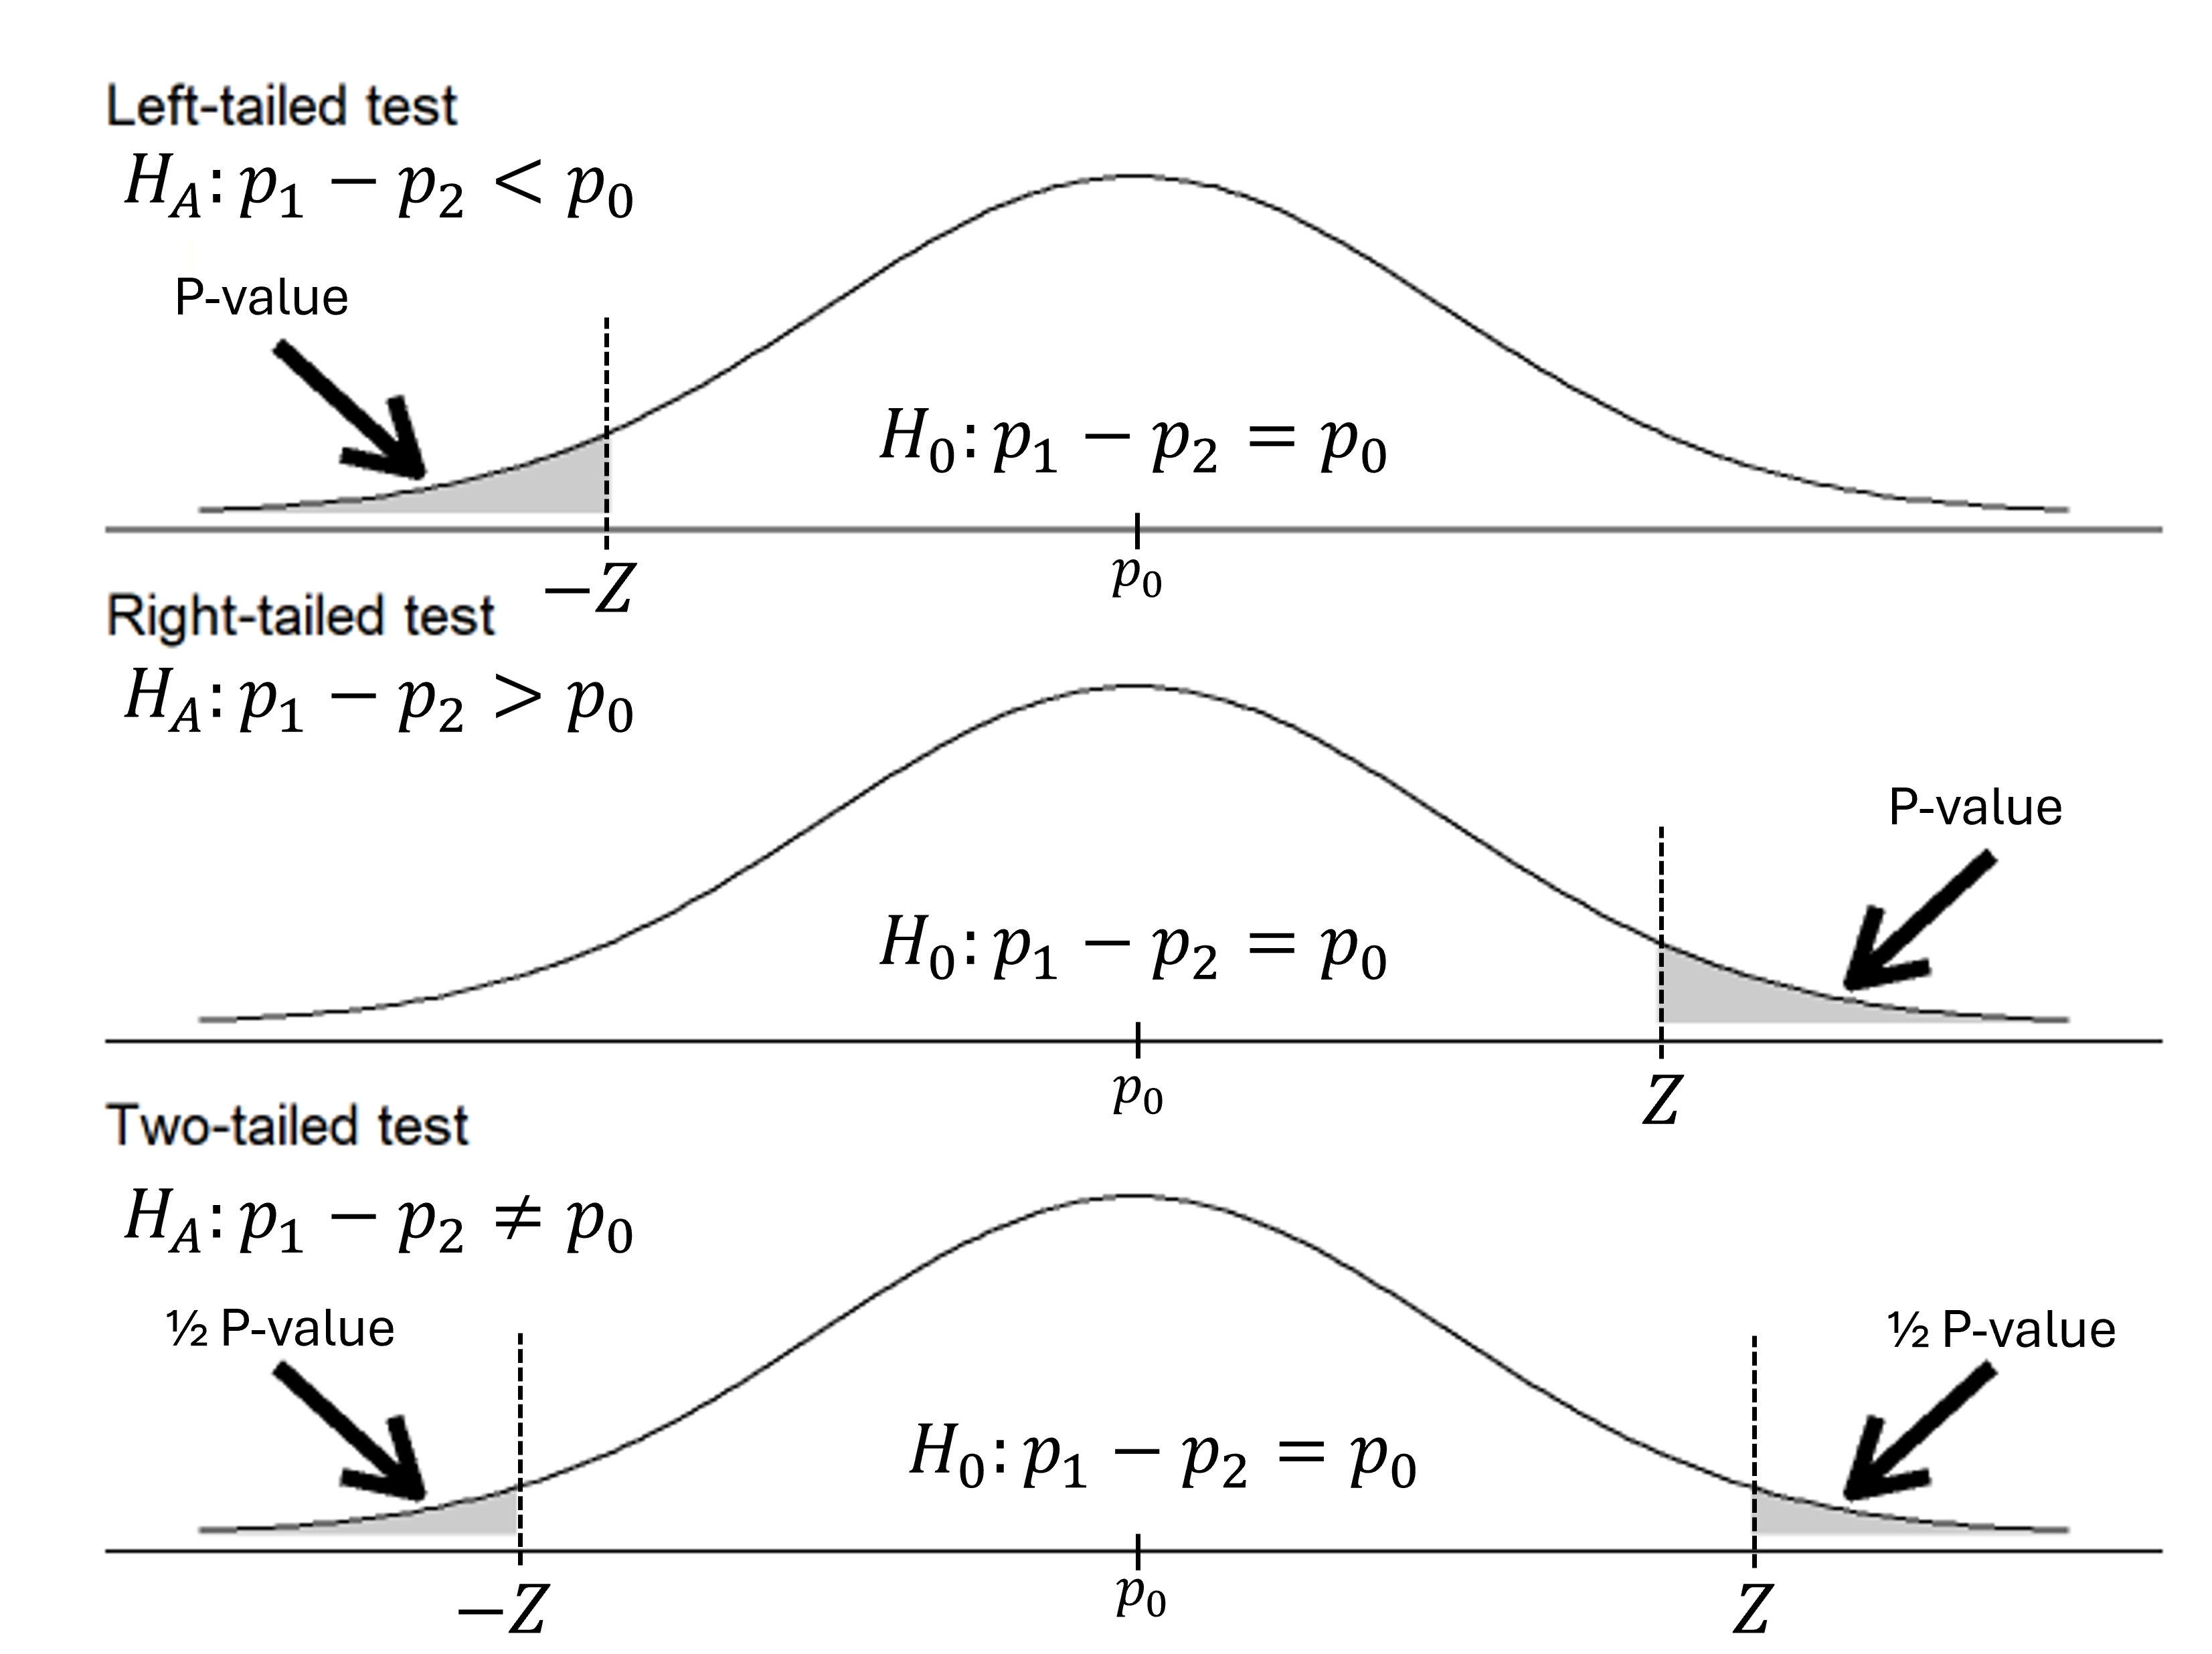
\includegraphics{cheatsheet_files/mediabag/two-sample-prop-test.png}

The test statistic \(Z\) (the \(Z\)-statistic) calculates how many
standard errors (\(\text{SE}_{\hat{p}_1-\hat{p}_2}\)) away from the null
hypothesis \(p_0\) that the observed statistic \(\hat{p}_1-\hat{p}_2\)
is.

\[
Z=\frac{(\hat{p}_1-\hat{p}_2)-p_0}{\text{SE}_{\hat{p}_1-\hat{p}_2}=
\begin{cases}
\frac{(\hat{p}_1-\hat{p}_2)-p_0}{\sqrt{\frac{\hat{p}_1(1-\hat{p}_1)}{n_1}+\frac{\hat{p}_2(1-\hat{p}_2)}{n_2}}}
\end{cases}
\]

The \(Z\)-statistic is used to find the probability of your sample
having the mean proportion \(\hat{p}\) if the null distribution
\(\text{N}\left(p_0, \text{SE}_{\hat{p}_0}\right)\) were the ``true''
distribution in your population.

The probability of the sample statistic \(\hat{p}\) under the null
hypothesis \(p=p_0\) is calculated from the \(Z\) distribution in R
using the function \texttt{pnorm()}. This function takes the test
statistic \(Z\) (called \texttt{q} or quantile in R), the \texttt{mean}
(default = 0), and the standard deviation (\texttt{sd}, default = 1) as
parameters. This probability is known as the p-value.

\begin{Shaded}
\begin{Highlighting}[]
\CommentTok{\# left{-}tailed hypothesis test}
\FunctionTok{pnorm}\NormalTok{(}\SpecialCharTok{{-}}\NormalTok{Z)}

\CommentTok{\# right{-}tailed hypothesis test}
\FunctionTok{pnorm}\NormalTok{(Z, }\AttributeTok{lower.tail=}\NormalTok{F)}

\CommentTok{\# two{-}tailed hypothesis test}
\FunctionTok{pnorm}\NormalTok{(}\SpecialCharTok{{-}}\NormalTok{Z)}\SpecialCharTok{*}\DecValTok{2}
\FunctionTok{pnorm}\NormalTok{(Z, }\AttributeTok{lower.tail=}\NormalTok{F)}\SpecialCharTok{*}\DecValTok{2}
\FunctionTok{pnorm}\NormalTok{(}\SpecialCharTok{{-}}\NormalTok{Z)}\SpecialCharTok{+}\FunctionTok{pt}\NormalTok{(Z, }\AttributeTok{lower.tail=}\NormalTok{F)}
\end{Highlighting}
\end{Shaded}

A small p-value indicates that the probability of taking a sample of
size \(n\) with your observed sample proportion \(\hat{p}\) from the
null sampling distribution
\(\hat{p}_0 \sim \text{N}\left(p_0, \text{SE}_{\hat{p}_0}\right)\) is
very low.

If the p-value for your \(Z\)-statistic is less than your significance
threshold \(\alpha\) (i.e.~the Type I Error Rate), this is evidence that
the null hypothesis \(H_0 \colon p=p_0\) is not true. Reject the null
hypothesis \(H_0\) and accept the alternate hypothesis \(H_A\).

If the p-value for your \(Z\)-statistic is greater than \(\alpha\), this
is not sufficient evidence against the null hypothesis
\(H_0 \colon p=p_0\). You fail to reject the null hypothesis \(H_0\).




\end{document}
